% !TEX program = xelatex
\documentclass[a4paper,10pt]{article}
\usepackage[UTF8]{ctex}
\usepackage[top=10mm,bottom=10mm,left=12mm,right=12mm]{geometry}
\usepackage{amsmath,amssymb,bm}
\usepackage{array,tabularx,longtable,booktabs}
\usepackage[dvipsnames]{xcolor}
\usepackage{enumitem}
\usepackage{needspace}
\usepackage{hyperref}
\usepackage{graphicx}
\hypersetup{colorlinks=true,linkcolor=blue,urlcolor=blue}
\pagestyle{plain}
\setlength{\parindent}{0pt}
\setlength{\parskip}{2pt}
\setlist[itemize]{leftmargin=1.2em,itemsep=1pt,topsep=2pt}
\definecolor{deep}{HTML}{16324F}
\definecolor{bluea}{HTML}{0B5CAD}
\definecolor{reda}{HTML}{B42318}
\definecolor{greena}{HTML}{087443}
\definecolor{orangea}{HTML}{B54708}
\newcommand{\chap}[1]{\par\vspace{10pt}{\Huge\bfseries\color{deep} #1}\par\vspace{3pt}\hrule height .7pt\vspace{5pt}}
\newcommand{\qitem}[5]{%
\Needspace{6\baselineskip}
\vspace{3pt}
{\Large\bfseries\color{deep} #1}\quad{\bfseries\color{orangea}#2}\par
\textbf{题目：}#3\par
\textbf{答题骨架：}#4\par
\textbf{必写关键词：}{\color{bluea}#5}\par
\vspace{2pt}\hrule height .25pt
}
\newcommand{\warn}[1]{{\bfseries\color{reda}#1}}

\begin{document}
\begin{center}
{\Huge\bfseries 殷雅俊风格 100 份针对性训练题}\\[4pt]
{\Large 根本性证明 / 三方面分析 / 对称性 / 微元法 / 概念纠错}\\[4pt]
{\large 每份含题目、答题骨架、必写关键词；用于开卷考场快速迁移。}
\end{center}
\hrule
\vspace{6pt}

\textbf{定位：}这不是普通题库，而是针对“重概念根源、重证明、重几何协调-物理本构-静力平衡、重对称性与微元法”的训练册。每份题都要求你写出逻辑链，而不是只背公式。

\textbf{使用方法：}
\begin{itemize}
  \item 考前：按章节顺序扫一遍，记每类题的“第一句话”和“必写关键词”。
  \item 考场：遇到证明/简答题，优先翻第 1、5 章；遇到超静定/综合题，翻第 2、4 章；遇到微分方程或圆环/梁问题，翻第 3 章。
  \item 答题：先写概念和模型，再写公式；证明题必须出现逻辑链。
\end{itemize}

\section*{总目录}
\begin{longtable}{@{}p{0.12\linewidth}p{0.30\linewidth}p{0.50\linewidth}@{}}
\toprule
\textbf{编号} & \textbf{模块} & \textbf{训练目标}\\
\midrule
01-25 & 概念追溯与根本性证明 & 防简答、证明、概念解释题。\\
26-50 & 三方面分析法 & 强制写几何协调、物理本构、静力平衡。\\
51-70 & 对称性与微元法 & 防圆环、曲杆、梁微分方程、微元平衡题。\\
71-90 & 综合计算变式 & 把基础公式接成完整解题链。\\
91-100 & 短答纠错与反例 & 防选择、填空、解释、判断题。\\
\bottomrule
\end{longtable}

\chap{一、概念追溯与根本性证明 25 份}

\qitem{01}{剪应力互等定理}
{取一个微小正六面体，证明互相垂直两截面上的剪应力成对相等。}
{1. 取微元体为 \(dx \times dy \times dz\)，在其垂直于 \(x\) 轴和 \(y\) 轴的面上分别受剪应力 \(\tau_{xy}\) 和 \(\tau_{yx}\)。\\
2. 考虑微元体绕 \(z\) 轴的力矩平衡：
   \(\sum M_z = 0 \implies (\tau_{xy} \cdot dy \, dz) \cdot dx - (\tau_{yx} \cdot dx \, dz) \cdot dy = 0\)。\\
3. 两边同除以微元体积 \(dx \, dy \, dz\)，即得：\(\tau_{xy} = \tau_{yx}\)。同理可证 \(\tau_{yz} = \tau_{zy}\)，\(\tau_{zx} = \tau_{xz}\)。}
{微元体；力矩平衡；力矩臂；剪应力互等}

\qitem{02}{为什么强度看应力}
{说明为什么构件强度问题不能只看外力大小，而必须转化为截面应力，并阐明强度失效的本质。}
{1. \textbf{强度失效本质}：构件因受力过大导致材料发生塑性变形或断裂破坏（应力超过材料极限）。例如，“这根钢缆可以吊起来十个集装箱”就是典型的强度描述，其极限状态为材料断裂。\\
2. \textbf{应力是内力密度}：外力由截面传递形成内力（合力），内力除以截面积得到应力，应力物理上即为“内力的分布密度”。\\
3. \textbf{危险点控制原则}：构件的破坏由局部最薄弱的危险点控制。即使内力相同，若截面积小或有应力集中，危险点应力就会超标导致断裂。故强度校核必须看危险点的最大应力是否满足 \(\sigma_{\max} \le [\sigma]\)。}
{强度失效；内力密度；截面法；危险点；钢缆吊重}

\qitem{03}{刚度为什么看位移}
{解释“刚度”与“强度”的本质区别，说明刚度失效的含义，并阐明为什么刚度校核要看位移或转角。}
{1. \textbf{刚度失效本质}：构件在荷载下产生过大弹性变形，导致功能失效（材料未坏）。例如，自行车轱辘加轮辐，或 4090 显卡加支架防止 PCB 板变弯，都是为了提高刚度防止过大位移。\\
2. \textbf{刚与钢的区别}：“钢”是一类碳铁合金材料；“刚”是结构抵抗弹性变形的能力（stiffness），二者本质不同。\\
3. \textbf{校核位移与转角}：刚度限制的是位移（如挠度 \(w \le [w]\)）或转角（如扭转角 \(\theta \le [\theta]\)）。}
{刚度失效；位移约束；轮辐刚度；显卡支架；刚与钢}

\qitem{04}{稳定为什么不是强度}
{解释压杆稳定问题为什么不能只用 \(\sigma=P/A\le[\sigma]\) 判断，并举例说明。}
{1. \textbf{失效物理本质不同}：强度失效是受力过大导致破坏（应力超极限）；稳定失效是由于受压导致平衡状态的突变（从直立平衡突变为弯曲平衡）。例如，烧烤签子戳到墙上变弯了，就是受压失稳，属于稳定性失效。\\
2. \textbf{影响因素不同}：强度仅与截面积 \(A\) 及材料强度有关；稳定性还与杆长 \(L\)、边界约束条件（\(\mu\)）及抗弯刚度 \(EI\) 密切相关，失稳往往发生在应力远低于屈服极限时。\\
3. \textbf{计算公式不同}：强度用 \(\sigma = P/A \le [\sigma]\)；稳定用 \(P \le P_{cr}/F_s\)。}
{平衡状态突变；临界载荷；屈曲；失稳；烧烤签子}

\qitem{05}{柔度系数的定义}
{说明柔度系数 \(\delta_{ij}\) 为什么定义为“在 \(j\) 处单位广义力引起的 \(i\) 处广义位移”。}
{1. \textbf{物理基础（线性小变形）}：在小变形和线弹性假设下，结构上任意点 \(i\) 的位移 \(\Delta_i\) 与引起它的外载荷 \(P_j\) 满足严格的线性比例关系：\(\Delta_i = \delta_{ij} P_j\)。\\
2. \textbf{比例系数的提取}：为了确定比例常数 \(\delta_{ij}\)，人为令作用在 \(j\) 处的力 \(P_j = 1\)（即单位力）。此时得到的位移 \(\Delta_i\) 在数值上即等于该比例系数 \(\delta_{ij}\)。\\
3. \textbf{多载荷叠加性}：当结构同时承受多个外载荷 \(P_1, P_2, \dots, P_n\) 时，根据位移的线性叠加原理，\(i\) 处的总位移为各个力单独作用引起的位移之和：\(\Delta_i = \sum_{j=1}^n \delta_{ij} P_j\)。这也是超静定力法方程的数学根基。}
{单位广义力；广义位移；线性叠加；柔度矩阵}

\qitem{06}{刚度与柔度互逆}
{从线性关系角度说明刚度矩阵与柔度矩阵为什么互为逆矩阵。}
{1. \textbf{基本物理方程}：在线弹性多自由度系统中，力向量 \(\bm{P} = [P_1, P_2, \dots, P_n]^T\) 和位移向量 \(\bm{\Delta} = [\Delta_1, \Delta_2, \dots, \Delta_n]^T\) 的对应关系可以从两个相反的视角描述。\\
2. \textbf{柔度方程（以力求位移）}：将位移表达为力的线性组合，引入柔度矩阵 \(\bm{\delta}\)：
   \[ \bm{\Delta} = \bm{\delta} \bm{P} \]
3. \textbf{刚度方程（以位移求力）}：将力表达为位移的线性组合，引入刚度矩阵 \(\bm{k}\)：
   \[ \bm{P} = \bm{k} \bm{\Delta} \]
4. \textbf{互逆性证明}：将刚度方程代入柔度方程，有 \(\bm{\Delta} = \bm{\delta} (\bm{k} \bm{\Delta}) = (\bm{\delta} \bm{k}) \bm{\Delta}\)。由于此式对任意位移向量均成立，故必有系数矩阵乘积为单位阵：\(\bm{\delta} \bm{k} = \bm{I}\)，即 \(\bm{k} = \bm{\delta}^{-1}\)（或 \(\bm{\delta} = \bm{k}^{-1}\)）。这说明刚度与柔度在描述结构抗变形特性时体征上互为逆表征。}
{线性系统；位移向量；力向量；互逆}

\qitem{07}{功互等定理（Betti定理）}
{证明或解释线弹性结构中两组外力的功互等关系。}
{1. \textbf{状态定义}：状态1受力系 \(P_i\) 产生位移 \(\Delta_i\)；状态2受力系 \(P_j^*\) 产生位移 \(\Delta_j^*\)；\\
2. \textbf{功互等公式}：第一组力在第二组位移上作功为 \(W_{12} = \sum P_i \Delta_i^*\)；第二组力在第一组位移上作功为 \(W_{21} = \sum P_j^* \Delta_j\)；\\
3. \textbf{定理表述}：\(W_{12} = W_{21} \implies \sum P_i \Delta_i^* = \sum P_j^* \Delta_j\)。}
{线弹性；外力功；状态位移；功互等}

\qitem{08}{位移互等定理}
{由功互等定理证明 Maxwell 位移互等定理 \(\delta_{ij}=\delta_{ji}\)。}
{1. \textbf{状态定义}：状态1在位置 \(i\) 施加单位力 \(P_i=1\)，位置 \(j\) 产生位移 \(\delta_{ji}\)；状态2在位置 \(j\) 施加单位力 \(P_j=1\)，位置 \(i\) 产生位移 \(\delta_{ij}\)；\\
2. \textbf{应用功互等}：\(W_{12} = W_{21} \implies P_i \cdot \delta_{ij} = P_j \cdot \delta_{ji}\)；\\
3. \textbf{结论}：因 \(P_i = P_j = 1\)，直接得 \(\delta_{ij} = \delta_{ji}\)。}
{单位力；功互等；柔度系数对称；位移互等}

\qitem{09}{单位载荷法本质}
{解释单位载荷法为什么可以求某一点某方向的位移。}
{1. \textbf{虚功原理本质}：单位载荷法（又称图乘法的基础）是虚功原理在变形体上的具体应用。设真实状态（位移状态）在力系作用下产生真实位移 \(\Delta\)，而虚拟状态是在求位移方向施加一个单位力 \(\bar{P} = 1\)。\\
2. \textbf{虚功方程建立}：外虚功为虚拟力 \(\bar{P}=1\) 在真实位移 \(\Delta\) 上作的功：\(W_{\text{ex}} = 1 \cdot \Delta\)。内虚功为虚拟状态引起的内力（如弯矩 \(\bar{M}(x)\)）在真实状态产生的微元变形（如 \(\mathrm{d}\theta = \frac{M(x)}{EI}\mathrm{d}x\)）上作的功：\(W_{\text{in}} = \int_L \frac{M(x)\bar{M}(x)}{EI}\mathrm{d}x\)。\\
3. \textbf{最终公式}：由虚功原理 \(W_{\text{ex}} = W_{\text{in}}\)，直接得到目标位移：
   \[ \Delta = \int_L \frac{M(x)\bar{M}(x)}{EI}\mathrm{d}x + \int_L \frac{N(x)\bar{N}(x)}{EA}\mathrm{d}x + \dots \]
   这表明单位力不仅给出了位移量，还作为“传感器”提取出了结构变形对目标位移的贡献。}
{虚功；单位力；真实内力；虚内力}

\qitem{10}{卡氏第二定理与多变形模式下应变能的正交叠加性}
{证明卡氏第二定理中应变能对力的偏导数等于载荷方向的位移；并剖析当结构同时发生弯曲和扭转时，总应变能 \(U\) 是否可以直接写为弯曲应变能 \(U_M\) 和扭转应变能 \(U_T\) 的简单代数相加，阐明其背后的正交叠加性物理条件。}
{1. \textbf{卡氏第二定理证明（偏导推导）}：\\
   对于线弹性系统，外力缓慢加载时外力功等于应变能：\(U = W = \frac{1}{2} \sum P_i \Delta_i\)，其中位移为 \(\Delta_i = \sum \delta_{ij} P_j\)。
   对应变能对某一力 \(P_i\) 求偏导有：
   \[ \frac{\partial U}{\partial P_i} = \frac{1}{2} \Delta_i + \frac{1}{2} \sum_{j=1}^n P_j \frac{\partial \Delta_j}{\partial P_i} = \frac{1}{2} \Delta_i + \frac{1}{2} \sum_{j=1}^n P_j \delta_{ji} \]
   由 Maxwell 位移互等定理有 \(\delta_{ji} = \delta_{ij}\)，代入上式有 \(\sum P_j \delta_{ij} = \Delta_i\)。
   两项相加即得：\(\frac{\partial U}{\partial P_i} = \frac{1}{2} \Delta_i + \frac{1}{2} \Delta_i = \Delta_i\)。\\
2. \textbf{多变形模式下的应变能叠加与正交性条件}：\\
   - \textbf{简单代数相加的条件}：只有当不同的变形模式（如弯曲和扭转）在截面上产生的\textbf{应力场在应变能积分中是正交（不相干）的}，总应变能才可以简单代数相加：\(U = U_M + U_T\)。\\
   - \textbf{物理剖析}：弯曲产生截面轴向正应力 \(\sigma_x\)，而扭转产生截面切向剪应力 \(\tau\)。总应变能密度为 \(u = \frac{\sigma_x^2}{2E} + \frac{\tau^2}{2G}\)。由于正应变能和剪切应变能是独立由不同的弹性模量（\(E\) 与 \(G\)）及独立的应力分量决定的，它们在积分中没有交叉耦合项（即无 \(\sigma_x \cdot \tau\) 项）。因此，弯扭组合时的总应变能可以直接代数相加：
     \[ U = \int_L \frac{M^2(x)}{2EI} \mathrm{d}x + \int_L \frac{T^2(x)}{2GI_p} \mathrm{d}x \]
   - \textbf{反例（非正交）}：若系统在同一个方向受到两个独立的载荷 \(P_1, P_2\) 产生同一变形模式（如均为弯弯矩），弯矩为 \(M = M_1 + M_2\)，则应变能中包含交叉相乘项 \(M_1 M_2\)，此时总应变能 \(U \neq U_1 + U_2\)，必须考虑耦合功。}
{卡氏定理；位移互等；应变能正交性；无耦合项；弯扭相加}

\qitem{11}{弯曲正应力公式来源}
{从平截面假设推导纯弯曲正应力 \(\sigma=My/I\)。}
{1. \textbf{几何关系（平截面假设）}：梁弯曲后，横截面保持为平面并旋转一角度。由此推得纵向纤维的应变 \(\varepsilon\) 与距中性轴的距离 \(y\) 成正比，与曲率半径 \(\rho\) 成反比：\(\varepsilon = y / \rho\)。\\
2. \textbf{物理关系（胡克定律）}：在线弹性单向应力状态下，正应力为：\(\sigma = E \varepsilon = E \frac{y}{\rho}\)。\\
3. \textbf{静力平衡关系}：
   - 轴力合力为零：\(F_N = \int_A \sigma \mathrm{d}A = \frac{E}{\rho}\int_A y \mathrm{d}A = 0 \implies S_z = 0\)（确定中性轴过形心）。
   - 弯矩平衡：\(M = \int_A \sigma y \mathrm{d}A = \frac{E}{\rho}\int_A y^2 \mathrm{d}A = \frac{E I_z}{\rho}\)，由此解出曲率 \(\frac{1}{\rho} = \frac{M}{EI_z}\)。\\
4. \textbf{最终公式}：将曲率代回物理关系，即得弯曲正应力公式：\(\sigma = \frac{M y}{I_z}\)。}
{平截面；中性轴；胡克定律；弯矩平衡}

\qitem{12}{中性轴为什么过形心}
{说明纯弯曲时中性轴为什么通过截面形心。}
{1. 纯弯曲梁横截面上无轴力，故总轴力合力为零（静力平衡）：$F_N = \int_A \sigma \mathrm{d}A = 0$。\\ 2. 弯曲正应力与中性轴距离 $y$ 成正比（$\sigma = k \cdot y = \frac{E}{\rho}y$）。\\ 3. 代入积分有 $F_N = \int_A k \cdot y \mathrm{d}A = k \int_A y \mathrm{d}A = 0$。由于梁发生弯曲，比例系数 $k \neq 0$，因此静矩 $\int_A y \mathrm{d}A = 0$。\\ 4. 由形心定义 $y_c = \frac{\int_A y \mathrm{d}A}{A} = 0$，说明形心到中性轴的距离为 0，即中性轴必过形心。\\ \warn{【物理注：因为横截面垂直于梁的轴线，故垂直于截面的正应力 $\sigma$ 即为轴向压强，微元面积 $\mathrm{d}A$ 上的微元力 $\mathrm{d}F_N = \sigma \mathrm{d}A$ 沿轴线方向，积分即得总轴向力 $F_N$。右图为官方课件图：$z$ 轴为中性轴，箭头代表正应力，弯矩为 $M_z$。】} \\ \begin{center}\includegraphics[width=0.32\textwidth]{beam_cross_section.png} \hfill \includegraphics[width=0.58\textwidth]{beam_shear_distribution.png}\end{center}}
{无轴力；正应力合力；一次矩；形心}

\qitem{13}{截面系数的意义}
{解释截面系数 \(W=I/y_{\max}\) 为什么能衡量抗弯能力。}
{1. \textbf{定义与公式}：纯弯曲梁横截面上最大正应力为 \(\sigma_{\max} = \frac{M y_{\max}}{I} = \frac{M}{W}\)。\\
2. \textbf{物理意义}：在弯矩 \(M\) 相同的情况下，\(W\) 越大，最大拉应力和压应力 \(\sigma_{\max}\) 就越小。因此，\(W\) 是一个纯粹的几何描述量，直接表征了横截面抵抗弯曲正应力破坏的能力。}
{最大纤维；抗弯能力；截面优化}

\qitem{14}{圆轴扭转公式来源}
{从圆轴扭转的“平截面假设”及“圆截面保持平面且无半径伸缩假设”，推导剪应力公式 \(\tau=\frac{T\rho}{I_p}\) 的三个基本关系（几何、物理、平衡关系），并解释平截面假设的物理图景。}
{1. \textbf{平截面假设的物理图景}：圆轴扭转时，任意两个相邻横截面之间仅发生相对旋转，每个横截面像一个刚性圆盘一样绕轴线旋转。变形后，横截面保持为平面，截面形状和半径长度均不发生改变，且横截面上的半径变形后仍保持为直射线。这保证了变形前后截面无面外位移（即无轴向翘曲）。\\
2. \textbf{三大关系推导}：
   \begin{itemize}
     \item \textbf{几何关系}：设两相邻截面间距为 \(\mathrm{d}x\)，相对转角为 \(\mathrm{d}\phi\)。在半径 \(\rho\) 处的微元体，其剪切角（剪应变）为圆弧长除以轴向长度：
           \[ \gamma = \frac{\rho \cdot \mathrm{d}\phi}{\mathrm{d}x} = \rho \phi' \quad (\phi' \text{ 为单位长度转角，常数}) \]
     \item \textbf{物理关系（胡克定律）}：由剪切胡克定律，剪应力与剪应变成正比：
           \[ \tau = G \gamma = G \rho \phi' \quad (\text{剪应力沿半径线性分布}) \]
     \item \textbf{平衡关系}：横截面上各微元剪应力对轴线产生的合力矩必须等于外力矩 \(T\)：
           \[ T = \int_A \tau \cdot \rho \, \mathrm{d}A = \int_A (G \rho \phi') \rho \, \mathrm{d}A = G \phi' \int_A \rho^2 \mathrm{d}A = G \phi' I_p \]
           其中 \(I_p = \int_A \rho^2 \mathrm{d}A\) 为极惯性矩。
   \end{itemize}
3. \textbf{最终公式}：由平衡关系得 \(\phi' = \frac{T}{G I_p}\)，代回物理关系即得：\(\tau = \frac{T\rho}{I_p}\)。}
{平截面假设；剪应变；剪切胡克定律；极惯性矩；扭矩平衡}

\qitem{15}{非圆截面扭转与翘曲}
{说明矩形截面等非圆截面扭转时，为什么“平截面假设”失效？其横截面会发生什么物理变形（翘曲）？其剪应力分布有何特点？最大剪应力发生在什么位置？}
{1. \textbf{平截面假设失效与翘曲（Warping）}：圆轴由于轴对称性，变形后横截面保持为平面。而对于矩形等非圆截面，如果各横截面仍保持平面并旋转，其边界处的剪应力将无法满足自由表面的边界条件（例如，矩形角点处的剪应力在两个相交的外表面上必须为 0，但若保持平面则角点应变最大，产生矛盾）。因此，非圆截面扭转时横截面必然发生面外位移，即\textbf{翘曲}（例如筷子或矩形条被扭转时，原本平齐的截面会变成弯曲的三维曲面）。\\
2. \textbf{应力分布特点与零应力位置}：
   \begin{itemize}
     \item 矩形截面的四个角点（Corner）由于处于互成直角的两个自由表面交界处，其剪应力必定为 \textbf{0}。
     \item 截面形心处的剪应力也为 \textbf{0}。
   \end{itemize}
3. \textbf{最大剪应力发生位置}：
   \begin{itemize}
     \item \textbf{最大剪应力}并不发生在距离形心最远的角点，而是发生在\textbf{长边的中点}（即最靠近形心的长外边缘中点）。
     \item \textbf{次大剪应力}发生在短边的中点。
     \item 沿矩形中心线（对称轴），剪应力大致呈非线性分布，在边缘中点达到最大，向中心逐渐减小至 0。
   \end{itemize}}
{非圆截面；平截面失效；翘曲；自由边界条件；长边中点}

\qitem{16}{弯曲剪切、剪应力公式推导与剪切翘曲}
{推导或解释梁弯曲剪应力公式 \(\tau=VQ/(Ib)\)（Jourawski 剪应力公式）的物理和数学来源；阐明在横向弯曲（有剪力 \(V \neq 0\)）时，梁的横截面“平截面假设”是否依然成立，并分析剪切翘曲的物理图景与剪应力沿高度的分布规律。}
{1. \textbf{微分段水平平衡与公式推导}：\\
   取长度为 \(\mathrm{d}x\) 的梁微段，在高度 \(y_1\) 处水平切开。由于弯矩沿轴向变化，左、右截面上的弯曲正应力不等，其差值在切开部分（面积为 \(A^*\)）产生不平衡轴向力：
   \[ \mathrm{d}F_N = \int_{A^*} \mathrm{d}\sigma \mathrm{d}A = \int_{A^*} \frac{\mathrm{d}M}{I} y \mathrm{d}A = \frac{\mathrm{d}M}{I} \int_{A^*} y \mathrm{d}A = \frac{\mathrm{d}M}{I} Q \]
   其中 \(Q = \int_{A^*} y \mathrm{d}A\) 为切开部分对中性轴的静矩。此轴向力差必须由水平切面上的剪力平衡，即 \(\tau \cdot b \cdot \mathrm{d}x = \mathrm{d}F_N\)。代入并利用 \(\frac{\mathrm{d}M}{\mathrm{d}x} = V\)（剪力与弯矩的微分关系）化简即得：\(\tau = \frac{VQ}{Ib}\)。\\
2. \textbf{弯曲剪切下的平截面假设失效与剪切翘曲}：\\
   - \textbf{平截面假设失效}：当梁受横向力弯曲时，横截面上必然存在剪力。由剪切胡克定律 \(\gamma = \tau/G\)，截面上必然发生剪变。由于剪应力 \(\tau\) 沿高度非均匀分布，导致剪切角（剪应变）\(\gamma\) 也非均匀。因此，\textbf{变形后的横截面不再保持为平面，而是发生面外弯曲位移}，称为\textbf{剪切翘曲}（Shear Warping）。\\
   - \textbf{变形图景与应力分布}：对矩形截面，中性轴处剪应力最大，其剪切角 \(\gamma\) 最大；上下外边缘剪应力为 0，剪切角 \(\gamma\) 也为 0。这导致截面在受剪弯曲后，中心凸出，边缘滞后，横截面呈 S 型弯曲曲面。\\
   - \textbf{考场防坑点}：虽然剪切翘曲导致平截面假设在力学上不再严格成立。但对细长梁（高跨比 \(h/L \ll 1\)），剪切变形引起的挠度占比极小，初等弯曲理论中通常依然近似采用平截面假设；而在短粗梁或薄壁构件中，则必须引入剪切变形修正。}
{正应力差；水平剪切平衡；静矩；平截面假设失效；剪切翘曲；细长梁近似}

\qitem{17}{莫尔圆的来源}
{证明平面应力状态下的应力变换公式在 \(\sigma-\tau\) 坐标系中是一个圆。}
{1. 移项：\(\sigma_\theta - \bar{\sigma} = \frac{\sigma_x-\sigma_y}{2}\cos 2\theta + \tau_{xy}\sin 2\theta\)，其中 \(\bar{\sigma}=\frac{\sigma_x+\sigma_y}{2}\)；\\
2. 联立剪应力公式：\(\tau_\theta = -\frac{\sigma_x-\sigma_y}{2}\sin 2\theta + \tau_{xy}\cos 2\theta\)；\\
3. 两式分别平方并相加，利用 \(\sin^2 2\theta + \cos^2 2\theta = 1\) 且交叉项抵消，得：\\
   \((\sigma_\theta - \bar{\sigma})^2 + \tau_\theta^2 = \left(\frac{\sigma_x-\sigma_y}{2}\right)^2 + \tau_{xy}^2\)；\\
4. 此即标准圆方程 \((x-x_0)^2+y^2=R^2\)，圆心为 \((\bar{\sigma}, 0)\)，半径为 \(R = \sqrt{\left(\frac{\sigma_x-\sigma_y}{2}\right)^2 + \tau_{xy}^2}\)。}
{应力变换；消去参数；圆心坐标；莫尔圆半径}

\qitem{18}{主应力为什么剪应力为零}
{说明主平面上剪应力为零的数学和物理含义。}
{1. \textbf{主平面的数学定义}：主平面是法线方向与该面上所受的合应力方向完全平行的平面。这意味着该面上的合应力矢量 \(\bm{T}\) 只有法向分量，没有切向分量。\\
2. \textbf{特征值问题与对角化}：在三维应力状态下，设应力张量为 \(\bm{\sigma}\)。主方向 \(\bm{n}\) 满足特征值方程：\(\bm{\sigma} \bm{n} = \sigma \bm{n}\)。这说明在此方向上，面上受到的全应力向量完全沿着法向 \(\bm{n}\)。因此，截面剪应力（全应力减去正应力）在定义上必然为零：\(\tau = \|\bm{\sigma} \bm{n} - (\bm{n}^T \bm{\sigma} \bm{n})\bm{n}\| = 0\)。\\
3. \textbf{莫尔圆几何解释}：在平面应力莫尔圆上，主平面对应于圆与横坐标轴 \(\sigma\) 的交点（\(\tau = 0\)）。在这些交点上，剪应力值为零，正应力达到极值（最大主应力 \(\sigma_1\) 和最小主应力 \(\sigma_3\)）。}
{主方向；对角化；莫尔圆交点}

\qitem{19}{第三强度理论本质}
{解释最大剪应力理论（Tresca 屈服准则）的物理本质，说明为什么用主应力差作为相当应力，并给出其在一般应力状态和弯扭组合状态下的相当应力公式。}
{1. \textbf{物理本质}：最大剪应力理论认为，材料发生屈服是由最大剪应力达到某一极限值引起的，适用于塑性材料的剪切滑移失效。\\
2. \textbf{主应力差作为相当应力}：复杂应力状态下的最大剪应力为 \(\tau_{\max} = \frac{\sigma_1 - \sigma_3}{2}\)。单向拉伸屈服时，其主应力为 \(\sigma_1 = \sigma_s, \sigma_2 = \sigma_3 = 0\)，对应最大剪应力为 \(\tau_{\max}^0 = \frac{\sigma_s}{2}\)。屈服时满足 \(\tau_{\max} = \tau_{\max}^0 \implies \frac{\sigma_1 - \sigma_3}{2} = \frac{\sigma_s}{2}\)，即 \(\sigma_1 - \sigma_3 = \sigma_s\)。故定义相当应力为 \(\sigma_{eq3} = \sigma_1 - \sigma_3\)。强度条件为 \(\sigma_{eq3} \le [\sigma]\)。\\
3. \textbf{公式变形与应用}：平面应力异号时，公式化为 \(\sigma_{eq3} = \sqrt{\sigma_x^2 + 4\tau_{xy}^2}\)。在仅受弯矩 \(M\) 和扭矩 \(T\) 的圆轴危险点上，正应力 \(\sigma_x = \frac{M}{W_z}\)，剪应力 \(\tau_{xy} = \frac{T}{2W_z}\)，相当应力简化为：
   \[ \sigma_{eq3} = \frac{\sqrt{M^2 + T^2}}{W_z} \]}
{Tresca；最大剪应力；主应力差；屈服；单向拉伸对标；弯扭组合}

\qitem{20}{第四强度理论本质}
{解释形状改变比能理论（von Mises 屈服准则）的物理本质，说明为什么它适合塑性材料的屈服判断，并给出其在一般应力状态和弯扭组合状态下的相当应力公式。}
{1. \textbf{物理本质}：体积改变比能（静水压力）不引起塑性屈服，引起屈服的物理主导因素是形状改变比能（畸变能，即剪切变形能）。\\
2. \textbf{公式定义与定标}：复杂应力状态下的畸变能密度 \(u_d\) 达到单向拉伸屈服时的临界值 \(u_d^0\) 时材料发生屈服。通过畸变能等效，定义相当应力为：
   \[ \sigma_{eq4} = \sqrt{\frac{1}{2}\left[(\sigma_1-\sigma_2)^2 + (\sigma_2-\sigma_3)^2 + (\sigma_3-\sigma_1)^2\right]} \]
   强度条件为 \(\sigma_{eq4} \le [\sigma]\)。\\
3. \textbf{公式变形与应用}：平面应力分量下（\(\sigma_y = \sigma_z = 0\)）化为 \(\sigma_{eq4} = \sqrt{\sigma_x^2 + 3\tau_{xy}^2}\)。在仅受弯矩 \(M\) 和扭矩 \(T\) 的圆轴危险点上，正应力 \(\sigma_x = \frac{M}{W_z}\)，剪应力 \(\tau_{xy} = \frac{T}{2W_z}\)，相当应力简化为：
   \[ \sigma_{eq4} = \frac{\sqrt{M^2 + 0.75T^2}}{W_z} \]}
{畸变能；Mises；塑性屈服；相当应力；体积改变；弯扭组合}

\qitem{21}{Euler 压杆公式来源}
{从梁挠曲微分方程推导两端铰支压杆临界力。}
{1. \textbf{微小扰动几何分析}：设两端铰支直压杆受到轴向压力 \(P\)。当压力达到临界值时，由于微小扰动，杆件发生微小的侧向挠曲，挠曲线为 \(w(x)\)。\\
2. \textbf{建立弯矩与挠曲线微分方程}：在任意截面 \(x\) 处，压杆受力产生的弯矩为 \(M(x) = -P w(x)\)。代入挠曲线近似微分方程：
   \[ EI_z w''(x) = -M(x) \implies EI_z w''(x) + P w(x) = 0 \]
3. \textbf{通解与边界条件应用}：设 \(k^2 = P / (EI_z)\)，微分方程变形为 \(w'' + k^2 w = 0\)。其通解为 \(w(x) = A \sin(kx) + B \cos(kx)\)。
   - 边界条件 1（\(x=0\) 处铰支）：\(w(0) = 0 \implies B = 0\)。
   - 边界条件 2（\(x=L\) 处铰支）：\(w(L) = A \sin(kL) = 0\)。\\
4. \textbf{非零特征解与临界力}：若要压杆发生屈曲（即存在非零解 \(A \ne 0\)），则必须满足特征方程：\(\sin(kL) = 0 \implies kL = n\pi\)（\(n=1, 2, \dots\)）。一阶屈曲（最容易发生的屈曲形态，\(n=1\)）对应临界力为：
   \[ P_{\text{cr}} = k^2 EI_z = \frac{\pi^2 EI_z}{L^2} \]
   证毕。}
{微小扰动；非零解；边界条件；临界载荷}

\qitem{22}{等效长度系数意义}
{解释压杆长度系数 \(\mu\) 的物理意义。}
{1. \textbf{等效物理定义}：长度系数 \(\mu\) 使得 \(\mu L\) 成为压杆的等效计算长度。\(\mu L\) 物理上代表压杆在屈曲变形时，\textbf{相邻两个弯曲拐点（即弯矩为 0 的点）之间的距离}，这相当于一根两端铰支的欧拉压杆的有效变形长度。\\
2. \textbf{端部约束对失稳的影响}：
   - 约束越强，拐点间距越短，\(\mu\) 越小，抗失稳能力越强。例如：两端固定压杆的半波长度仅为杆长一半，\(\mu = 0.5\)。
   - 约束越弱，拐点间距越长，\(\mu\) 越大。例如：一端固定一端自由的压杆，等效于两倍长度的铰支杆，\(\mu = 2.0\)。\\
3. \textbf{临界力表达}：通用的欧拉公式为 \(P_{\text{cr}} = \frac{\pi^2 EI_z}{(\mu L)^2}\)，直观地说明了约束如何通过改变等效长度来决定稳定性。}
{计算长度；端部约束；屈曲半波}

\qitem{23}{平面应力与平面应变区别}
{解释为什么平面应力是 \(\sigma_z=0\)，平面应变是 \(\varepsilon_z=0\)。}
{1. \textbf{平面应力状态（薄板模型）}：适用于厚度远小于其长宽尺寸的薄板。由于薄板前、后两表面是自由表面，无外界横向荷载，因此在厚度方向（\(z\) 轴）各点受力极小：\(\sigma_z = \tau_{zx} = \tau_{zy} = 0\)。但此时轴向变形不为零（\(\varepsilon_z \neq 0\)），薄板在拉伸时由于泊松效应会变薄。\\
2. \textbf{平面应变状态（厚重构件模型）}：适用于沿 \(z\) 轴长度无限长、且横截面受力不随 \(z\) 轴变化的构件（如水坝、隧道管道）。由于纵向尺寸巨大，且两端受外界强烈约束限制其伸缩，导致轴向变形完全受限：\(\varepsilon_z = \gamma_{zx} = \gamma_{zy} = 0\)。但此时轴向应力不为零（\(\sigma_z \neq 0\)），约束反力在轴向产生了相当大的正应力。\\
3. \textbf{本构方程的差异}：在广义胡克定律中，二者常数的等效转换不同。例如，平面应变中的弹性模量需代换为 \(E' = \frac{E}{1-\nu^2}\)，泊松比代换为 \(\nu' = \frac{\nu}{1-\nu}\)。}
{自由表面；变形受限；广义胡克定律}

\qitem{24}{换算截面的本质}
{说明组合梁中为什么可以用 \(n=E_i/E_0\) 做换算截面。}
{1. \textbf{平截面假设与变形协调}：两种材料紧密粘结共同受弯时，交界面处无滑动，满足平截面假设。这意味着在高度为 \(y\) 处，无论属于哪种材料，其弯曲正应变是完全相同的：\(\varepsilon(y) = \kappa y\)。\\
2. \textbf{材料胡克定律的差异}：根据一维胡克定律，不同材料的应力与各自的弹性模量成正比：\(\sigma_1 = E_1 \varepsilon\)，\(\sigma_2 = E_2 \varepsilon\)。应力之比为弹性模量比：\(\sigma_1 / \sigma_2 = E_1 / E_2 = n\)。\\
3. \textbf{换算宽度的几何等效}：为了将双材料截面转化为单一材料（如材料 1），根据合弯矩等效：\(\mathrm{d}F = \sigma_2 \mathrm{d}A = \sigma_2 (b \mathrm{d}y) = (E_2 \varepsilon) (b \mathrm{d}y) = (E_1 \varepsilon) (n b \mathrm{d}y) = \sigma_1 (n b \mathrm{d}y)\)。这说明在计算惯性矩时，可将材料 2 的截面宽度乘以模量比 \(n\)，等效地替换为材料 1 的截面。这样便可使用普通单材料的弯曲公式计算应力和刚度。}
{完全粘合；应变协调；弹性模量比；等效刚度}

\qitem{25}{S-N 曲线的意义}
{解释疲劳题为什么不能只用静强度条件判断。}
{1. \textbf{疲劳破坏的物理机制}：构件在循环往复荷载（如拉压、弯曲循环）下，即使危险点处的最大工作应力低于材料的静强度极限 \(\sigma_s\)，经过一定次数的循环后也会发生突然断裂。其物理本质是微观裂纹在交变应力下逐渐萌生并缓慢扩展，最终导致截面削弱而突发脆性断裂。\\
2. \textbf{S-N 曲线的表达}：S-N 曲线是交变应力幅 \(S\)（或最大应力 \(\sigma_{\max}\)）与材料疲劳破坏时的循环寿命（次数）\(N\) 之间的关系曲线。随应力幅降低，疲劳寿命急剧增加。当应力幅低于“疲劳极限 \(\sigma_{-1}\)”时，材料在无限次循环（通常钢材定为 \(10^7\) 次）下也不会发生疲劳破坏。\\
3. \textbf{考场防坑点}：在设计旋转轴等承受循环应力的结构时，必须采用疲劳校核判据（如 Goodman 关系或 S-N 曲线），绝对不能直接使用静强度公式。}
{循环应力；应力幅；平均应力；寿命}

\chap{二、三方面分析法 25 份}

\qitem{26}{两端固定杆温升}
{一根等截面杆两端固定，温度升高 \(\Delta T\)。求杆内应力，并说明三方面分析。}
{1. \textbf{三方面分析法运用}：\\
   - \textbf{几何协调}：直杆两端受刚性墙限制，温升后热膨胀受阻，杆的总变形量必须为零：\(\Delta_T + \Delta_F = 0\)。\\
   - \textbf{物理本构}：温升引起的自由热变形量为 \(\Delta_T = \alpha \Delta T L\)，两端反力（压轴力 \(N\)）引起的轴向变形量为 \(\Delta_F = \frac{N L}{EA}\)。\\
   - \textbf{静力平衡}：直杆内各截面轴力相等，大小均等于端部支座的水平反力。\\
2. \textbf{联立求解内力与应力}：\\
   将本构代入几何方程有 \(\alpha \Delta T L + \frac{N L}{EA} = 0 \implies N = -EA \alpha \Delta T\)。\\
   两端固定的杆在温升时受压，其轴向热压应力为：\(\sigma = \frac{N}{A} = -E \alpha \Delta T\)。该应力仅与材料属性和温升值有关，与杆长无关。}
{几何协调；热变形；胡克定律；压应力}

\qitem{27}{有间隙的温度杆}
{一根等截面直杆两端被刚性挡板限制，左端与挡板有间隙 \(\delta\)。温升 \(\Delta T\) 后求是否接触及接触后的压应力 \(\sigma\)。}
{1. 先算自由热伸长：\(\Delta_T = \alpha \Delta T L\)。\\
2. 接触判定：若 \(\Delta_T \le \delta\)，杆与挡板未接触，无内应力（\(\sigma = 0\)）；若 \(\Delta_T > \delta\)，杆与挡板接触并受压。\\
3. 接触后应用“三方面分析法”：\\
   - \textbf{几何协调}：\(\Delta_T + \Delta_F = \delta\)（热膨胀量 \(\Delta_T\) 与受力变形量 \(\Delta_F\) 叠加等于间隙 \(\delta\)）。\\
   - \textbf{物理本构}：\(\Delta_T = \alpha \Delta T L\)，\(\Delta_F = \frac{\sigma L}{E}\)（\(E\) 为弹性模量，受压时应力 \(\sigma < 0\)）。\\
   - \textbf{静力平衡}：杆内轴力与挡板反力相等，应力沿轴向均匀分布。\\
4. 联立得：\(\alpha \Delta T L + \frac{\sigma L}{E} = \delta \implies \sigma = E\left(\frac{\delta}{L} - \alpha \Delta T\right)\)。}
{接触判断；几何协调；物理本构；热应力}

\qitem{28}{装配误差杆系}
{两根材料不同的杆通过刚性板连接，其中一根存在装配误差。求装配后杆力。}
{1. \textbf{变形协调方程（几何关系）}：设杆 1 比设计长度短了 \(\delta\)。在将它们强行装配并达到平衡后，刚性板会发生平移 \(u_y\) 和转角 \(\theta\)。各杆的实际伸长量 \(\Delta l_i\) 和缩短量与板的位移存在几何对应。为了使系统闭合，存在误差的杆件其位移协调需满足：\(\Delta l_1 - \Delta l_2 = \delta\)。\\
2. \textbf{本构方程（物理关系）}：由胡克定律，各杆的内力与弹性变形量成正比：\(\Delta l_i = \frac{N_i L_i}{E_i A_i}\)。\\
3. \textbf{静力平衡方程（静力关系）}：对刚性板列力与力矩平衡：\(\sum F_y = 0\) 和 \(\sum M = 0\)。\\
4. \textbf{综合求解}：将胡克定律代入位移协调方程中，化为未知杆力 \(N_i\) 的关系式，再与静力平衡方程联立，即可解出装配应力。}
{装配误差；刚性板；协调；平衡}

\qitem{29}{三杆悬挂刚性梁}
{刚性梁由三根竖杆悬挂，受集中力作用。求三杆内力。}
{1. \textbf{几何协调（刚体变形限制）}：由于悬挂梁为刚性梁（自身无弯曲变形），在挂上三根弹性杆并受外力作用后，刚性梁变形后的位置必然保持为一条直线。设三根竖直悬挂杆的间距对称分布，则三杆底端发生向下位移，根据相似三角形或直线方程，中杆变形与两侧杆变形满足对称或线性比例：\(\Delta l_1 + \Delta l_3 = 2\Delta l_2\)（若三杆等间距并联）。\\
2. \textbf{本构方程}：各杆的内力与变形量成正比：\(\Delta l_i = \frac{N_i L_i}{E_i A_i}\)。\\
3. \textbf{静力平衡}：对刚性梁建立静力学平衡：列出竖向力平衡 \(\sum F_y = 0\) 及绕某节点的力矩平衡 \(\sum M_A = 0\)。\\
4. \textbf{求解结论}：联立三者可解得三杆分配到的不均匀内力，进而可求出刚性梁的倾斜转角。}
{刚体转动；位移线性分布；三方面}

\qitem{30}{阶梯杆受轴力}
{阶梯杆由两段截面组成，端部受轴力。求总伸长与最大应力。}
{1. \textbf{分段内力求解}：首先使用截面法求出阶梯直杆各段截面上的内力（轴力 \(N_i\)）。注意，由于外载荷可能在阶梯交界处输入，各段轴力一般不相等。\\
2. \textbf{分段物理本构}：每一段由于截面积 \(A_i\)、长度 \(L_i\) 和材料 \(E_i\) 不同，其各自的伸长/缩短量为：\(\Delta l_i = \frac{N_i L_i}{E_i A_i}\)。\\
3. \textbf{变形协调（几何叠加）}：杆件的总轴向位移为各段轴向变形量的代数和：\(\Delta L = \sum_i \Delta l_i = \sum_i \frac{N_i L_i}{E_i A_i}\)。\\
4. \textbf{危险面应力校核}：在强度校核时，必须对每一段的截面应力进行检查，最大工作应力 \(\sigma_{\max} = \max_i \left( \frac{|N_i|}{A_i} \right)\) 发生在“内力较大”或“截面极细”的危险段上，需满足 \(\sigma_{\max} \le [\sigma]\)。}
{分段；轴力图；最大应力}

\qitem{31}{复合杆同伸长}
{钢杆和铝杆并联共同承受轴向力，求各自分担载荷。}
{1. \textbf{几何协调（等变形）}：当钢杆和铝杆并联共同承受外轴向力 \(P\) 时，由于两端板的限制，两杆在受拉时必须发生完全相同的伸长量：\(\Delta l_s = \Delta l_a = \Delta\)。\\
2. \textbf{物理本构（刚度分配）}：根据胡克定律，将各杆的轴力用公共位移 \(\Delta\) 表示：\(N_s = \frac{E_s A_s}{L}\Delta\)，\(N_a = \frac{E_a A_a}{L}\Delta\)。\\
3. \textbf{静力平衡（共同分担）}：两杆分担的轴力之和必须等于外载荷：\(N_s + N_a = P\)。\\
4. \textbf{求解分配公式}：代入平衡方程得 \(\left( \frac{E_s A_s}{L} + \frac{E_a A_a}{L} \right) \Delta = P\)，解出共同变形 \(\Delta\)。分担内力分别为：
   \[ N_s = P \cdot \frac{E_s A_s}{E_s A_s + E_a A_a}, \quad N_a = P \cdot \frac{E_a A_a}{E_s A_s + E_a A_a} \]
   这表明并联复合受力中，各构件按照其\textbf{拉压抗变刚度 \(EA\) 的比例}来分配载荷，较硬的材料（弹性模量 \(E\) 大或面积 \(A\) 大）会分担到更大的力。}
{并联杆；等伸长；刚度分配}

\qitem{32}{铆钉连接校核}
{一块钢板由铆钉连接，给定载荷、铆钉直径、板厚，校核剪切和挤压。}
{1. \textbf{剪切面判定（剪应力校核）}：确定受剪面的个数（单剪或双剪）。一个受剪面面积为 \(A_s = \frac{\pi d^2}{4}\)。由平衡条件，若有 \(n\) 个受剪面，平均剪应力为 \(\tau = \frac{P}{n A_s} \le [\tau]\)。\\
2. \textbf{挤压投影面判定（挤压应力校核）}：挤压接触面是半圆柱面。在工程上，为了简化，采用\textbf{沿力方向的投影面面积}计算：\(A_{bs} = d \cdot t\)（\(d\) 为铆钉直径，\(t\) 为受压钢板的厚度）。平均挤压应力为 \(\sigma_{bs} = \frac{P_{bs}}{A_{bs}} = \frac{P}{d \cdot t} \le [\sigma_{bs}]\)。\\
3. \textbf{钢板拉伸破坏校核（净截面）}：除校核铆钉外，还必须校核被连接钢板在铆钉孔处的强度。由于开孔导致截面积削弱，其净截面积为 \(A_{\text{net}} = (b - k d) \cdot t\)（\(k\) 为同截面排钉数）。钢板最大拉应力为 \(\sigma_{\max} = \frac{P}{A_{\text{net}}} \le [\sigma]\)。}
{单剪双剪；挤压面积；净截面}

\qitem{33}{圆轴两端固定中间扭矩}
{圆轴两端固定，中间施加扭矩。求两端反力矩。}
{1. \textbf{几何协调条件}：圆轴两端固定在刚性墙壁上，当在轴中某截面施加外扭矩 \(T\) 时，两端总的相对扭转角必须为零：\(\varphi_{AC} + \varphi_{CB} = 0\)。\\
2. \textbf{物理本构关系}：设左半段扭矩为 \(T_1\)，右半段扭矩为 \(T_2\)。由扭转角公式：\(\varphi_1 = \frac{T_1 L_1}{G I_{p1}}\)，\(\varphi_2 = \frac{T_2 L_2}{G I_{p2}}\)。\\
3. \textbf{静力平衡关系}：中间加载截面处的扭矩平衡要求左、右力矩代数和与外扭矩平衡：\(T_1 + T_2 = T\)。\\
4. \textbf{求解结论}：代入有 \(\frac{T_1 L_1}{G I_{p1}} + \frac{(T - T_1) L_2}{G I_{p2}} = 0\)。若两段为等直径同材料，可解得反力矩：
   \[ T_1 = T \cdot \frac{L_2}{L_1 + L_2}, \quad T_2 = T \cdot \frac{L_1}{L_1 + L_2} \]
   扭矩与各段的\textbf{扭转刚度成正比}分配。}
{扭转静不定；转角协调；扭矩图}

\qitem{34}{组合圆轴扭转}
{两段不同直径圆轴串联受扭矩，求最大剪应力和总转角。}
{1. \textbf{扭矩分布求解（平衡）}：首先通过截面法绘制圆轴的扭矩图，确定各段横截面受到的内力扭矩 \(T_i\)。\\
2. \textbf{各段扭转刚度（物理）}：根据各段的极惯性矩 \(I_{pi} = \frac{\pi d_i^4}{32}\) 和材料剪切模量 \(G_i\)，确定各段单位长度相对转角。\\
3. \textbf{变形叠加与总转角（几何）}：圆轴端部间的总扭转角为各段扭转角之和：\(\Phi = \sum_i \varphi_i = \sum_i \frac{T_i L_i}{G_i I_{pi}}\)。\\
4. \textbf{最大剪应力校核}：分别计算各段外表面的最大剪应力 \(\tau_{i,\max} = \frac{|T_i| d_i}{2 I_{pi}} = \frac{|T_i|}{W_{pi}}\)。危险点并不一定在最大扭矩段，因为细截面轴的 \(W_p\) 极小，必须对各段的最大剪应力进行全面评估。}
{分段扭转；极惯性矩；刚度}

\qitem{35}{矩形截面梁弯曲}
{简支矩形梁受集中力，求危险截面最大正应力。}
{1. \textbf{静力学内力分析（平衡）}：分析简支梁受力，求出支座反力，画出弯矩图，确定最大弯矩 \(M_{\max}\) 发生的危险截面位置。\\
2. \textbf{截面几何参数计算（几何）}：对高为 \(h\)、宽为 \(b\) 的矩形截面，其中性轴通过截面形心，惯性矩为 \(I_z = \frac{b h^3}{12}\)。偏离中性轴最远的上下边缘纤维距离为 \(y_{\max} = \frac{h}{2}\)。\\
3. \textbf{工作应力计算与校核（物理）}：弯曲正应力随高度线性分布，最大拉应力和压应力发生在截面最外侧表面的边缘纤维处：
   \[ \sigma_{\max} = \frac{|M_{\max}| y_{\max}}{I_z} = \frac{|M_{\max}|}{\left(\frac{b h^2}{6}\right)} = \frac{|M_{\max}|}{W_z} \]
   需满足强度条件 \(\sigma_{\max} \le [\sigma]\)。}
{弯矩图；截面惯性矩；危险点}

\qitem{36}{T 形截面弯曲}
{T 形截面梁受弯，求最大拉压应力。}
{1. \textbf{寻找中性轴位置（几何第一步）}：由于 T 形截面仅有一条对称轴，必须首先求出形心位置以确定中性轴位置：\(y_c = \frac{\sum A_i y_i}{\sum A_i}\)。\\
2. \textbf{惯性矩计算（几何第二步）}：利用平行移轴公式计算整个截面关于中性轴的惯性矩 \(I_z = \sum (I_{zi} + A_i d_i^2)\)。由于上下边缘不对称，距离中性轴的拉伸距离 \(y_t\) 和压缩距离 \(y_c\) 不相等。\\
3. \textbf{最大拉压应力比较（物理）}：根据危险弯矩的正负号：
   - 当弯矩使下边缘受拉时：最大拉应力为 \(\sigma_t = \frac{M y_{\text{lower}}}{I_z}\)；最大压应力为 \(\sigma_c = \frac{M y_{\text{upper}}}{I_z}\)。
   - 由于脆性材料的抗拉和抗压强度极限差别极大，必须在校核时同时满足 \(\sigma_t \le [\sigma_t]\) 和 \(\sigma_c \le [\sigma_c]\)。}
{形心；非对称截面；上下边缘比较}

\qitem{37}{偏心压缩矩形柱}
{矩形柱承受偏心压力，判断是否全截面受压并求最大应力。}
{1. \textbf{载荷等效简化（静力关系）}：作用在截面上某点 \((e_y, e_z)\) 的偏心压缩压力 \(P\)，可以等效化为作用于截面形心处的轴向压力 \(N = -P\) 以及绕两个主惯性轴的弯矩：\(M_z = P \cdot e_y\)，\(M_y = P \cdot e_z\)。\\
2. \textbf{应力叠加计算（物理关系）}：截面上任意点 \((y, z)\) 处的正应力为轴向压应力与弯曲正应力线性叠加：
   \[ \sigma(y, z) = -\frac{P}{A} \pm \frac{M_z y}{I_z} \pm \frac{M_y z}{I_y} = -\frac{P}{A} \left( 1 + \frac{A e_y y}{I_z} + \frac{A e_z z}{I_y} \right) \]
3. \textbf{全截面受压判定（截面核心）}：若要矩形柱完全不出现抗拉强度极弱的拉应力（即全截面 \(\sigma \le 0\)），偏心距必须控制在由极限直线包围的“截面核心（Core）”区域内。}
{截面核心；偏心压缩；无拉应力}

\qitem{38}{斜弯曲梁}
{梁在两个主惯性轴方向同时受弯，求截面角点应力。}
{1. \textbf{外力分解与内力分析（平衡）}：将作用在不平行于主惯性轴方向的斜向弯矩，分解为沿两个主惯性轴（\(y\) 轴和 \(z\) 轴）的分量，并分别绘制弯矩图，求得截面上的弯矩 \(M_y\) 和 \(M_z\)。\\
2. \textbf{双向弯曲正应力叠加（物理）}：在截面上任意点 \((y, z)\) 处，斜弯曲产生的正应力为两个方向弯曲正应力的叠加：
   \[ \sigma = \frac{M_z y}{I_z} + \frac{M_y z}{I_y} \]
3. \textbf{危险角点判定（几何）}：对矩形截面，最大应力必定发生在距离中性轴最远的四个角点（Corner）上。通过代入角点坐标，比较符号以确定最大拉应力和最大压应力。}
{双向弯曲；角点比较；符号}

\qitem{39}{弯扭组合圆轴与多向应力叠加}
{一根圆轴同时承受轴力 \(N\)、弯矩 \(M\)、扭矩 \(T\) 和剪力 \(V\)，试说明这些载荷产生的应力如何叠加？如何确定危险点的主应力和主平面方位？它们在强度设计中有什么用途？}
{1. \textbf{应力分量的全面叠加规律}：
   对于横截面上任意一点，各载荷产生的应力分量按其方向分别进行代数叠加：
   \begin{itemize}
     \item \textbf{轴向正应力 \(\sigma_x\)}：由轴力 \(N\) 和弯矩 \(M\) 叠加而成：
           \[ \sigma_x = \sigma_N \pm \sigma_M = \frac{N}{A} \pm \frac{M y}{I_z} \]
     \item \textbf{剪应力 \(\tau\)}：由扭矩 \(T\) 和横向剪力 \(V\) 叠加而成：
           \[ \tau = \tau_T \pm \tau_V = \frac{T \rho}{I_p} \pm \frac{V Q}{I_z b} \]
   \end{itemize}
   \warn{【考场注：通常在截面最外侧纤维（\(y = y_{\max}\)）处，弯曲正应力最大，但横向剪力的剪应力 \(\tau_V = 0\)（因为该处静矩 \(Q=0\)），竖向正应力 \(\sigma_y = 0\)（横向无受压）。此时该点处于平面应力状态，仅有正应力 \(\sigma_x\) 和扭转剪应力 \(\tau = \tau_T\)。代入主应力公式计算，由于三个主应力须按从大到小排序（\(\sigma_1 \ge \sigma_2 \ge \sigma_3\)），且面外主应力为 \(0\)，故：
    \[ \sigma_1 = \frac{\sigma_x}{2} + \sqrt{\left(\frac{\sigma_x}{2}\right)^2 + \tau^2} \ge 0, \quad \sigma_3 = \frac{\sigma_x}{2} - \sqrt{\left(\frac{\sigma_x}{2}\right)^2 + \tau^2} \le 0, \quad \sigma_2 = 0 \]
    （注意：由于 \(\sigma_1 \ge 0\) 且 \(\sigma_3 \le 0\)，面外主应力 \(0\) 必然处于二者之间，因此中间主应力 \(\sigma_2 = 0\)，而不是 \(\sigma_3 = 0\)。这样代入第三强度理论即得 \(\sigma_{eq3} = \sigma_1 - \sigma_3 = \sqrt{\sigma_x^2 + 4\tau^2}\)，与 Q19 一致）。其主平面方位满足 \(\tan(2\theta_0) = \frac{2\tau}{\sigma_x}\)。}
2. \textbf{在强度设计中的用途}：
   - 确定危险点的主应力后，可选用适当的强度理论评估其安全性。对于钢制圆轴等塑性材料，可用第三强度理论（相当应力 \(\sigma_{eq3} = \sqrt{\sigma_x^2 + 4\tau^2}\)）或第四强度理论（相当应力 \(\sigma_{eq4} = \sqrt{\sigma_x^2 + 3\tau^2}\)）进行校核（详见Q19和Q20的本质推导与圆轴简化公式）。
   - \textbf{预测破坏面角度}：
     \begin{itemize}
       \item 脆性材料（如铸铁）受扭转时，在 \(\theta_0 = 45^\circ\) 主平面上拉应力 \(\sigma_1\) 最大，由于其抗拉能力弱，故沿 \(45^\circ\) 螺旋面发生拉断破坏。
       \item 塑性材料（如低碳钢）受扭转时，最大剪应力发生在横截面上，故沿横截面剪断。
     \end{itemize}}
{抗弯截面系数；剪应力叠加；主应力；强度理论；主平面方位；破坏模式}

\qitem{40}{梁的剪应力与剪应力互等定理}
{阐明梁中剪应力的下标命名、分解本质、互等关系与物理表现，说明工字梁剪流分布。}
{1. \textbf{下标命名与分解}：剪应力 \(\tau_{ij}\) 中，\(i\) 为作用面法向，\(j\) 为受力方向。面上任意方向的剪应力矢量可通过正交分解表示为直角坐标分量（如横截面上的 \(\tau_{xy}, \tau_{xz}\)）。\\
2. \textbf{互等定理与物理表现}：由微元力矩平衡，有 \(\tau_{xy} = \tau_{yx}\)（\(\tau_{xz}=\tau_{zx}\)）。其中：
   \begin{itemize}
     \item \(\tau_{xy}\)：作用于横截面（法线 \(x\)），方向沿竖直（\(y\)），由横向剪力直接引起。
     \item \(\tau_{yx}\)：作用于纵向水平面（法线 \(y\)），方向沿轴向（\(x\)），表现为各水平层之间的\textbf{层间相对滑动趋势}（如木梁沿中性轴水平劈裂）。
   \end{itemize}
3. \textbf{工字截面“剪流”}：剪应力在截面中如水流汇合分布：
   \begin{itemize}
     \item \textbf{翼缘}：外表面无竖向剪应力，存在水平剪流 \(\tau_{xz}\) 自两侧流向腹板；
     \item \textbf{腹板}：水平剪流在此汇合，转化为竖向剪应力 \(\tau_{xy}\) 往下流动，承担了 95\% 以上的剪力。中性轴处最大：\(\tau_{\max} = \frac{V Q_{\max}}{I_z b}\)。
   \end{itemize}
   \begin{center}
     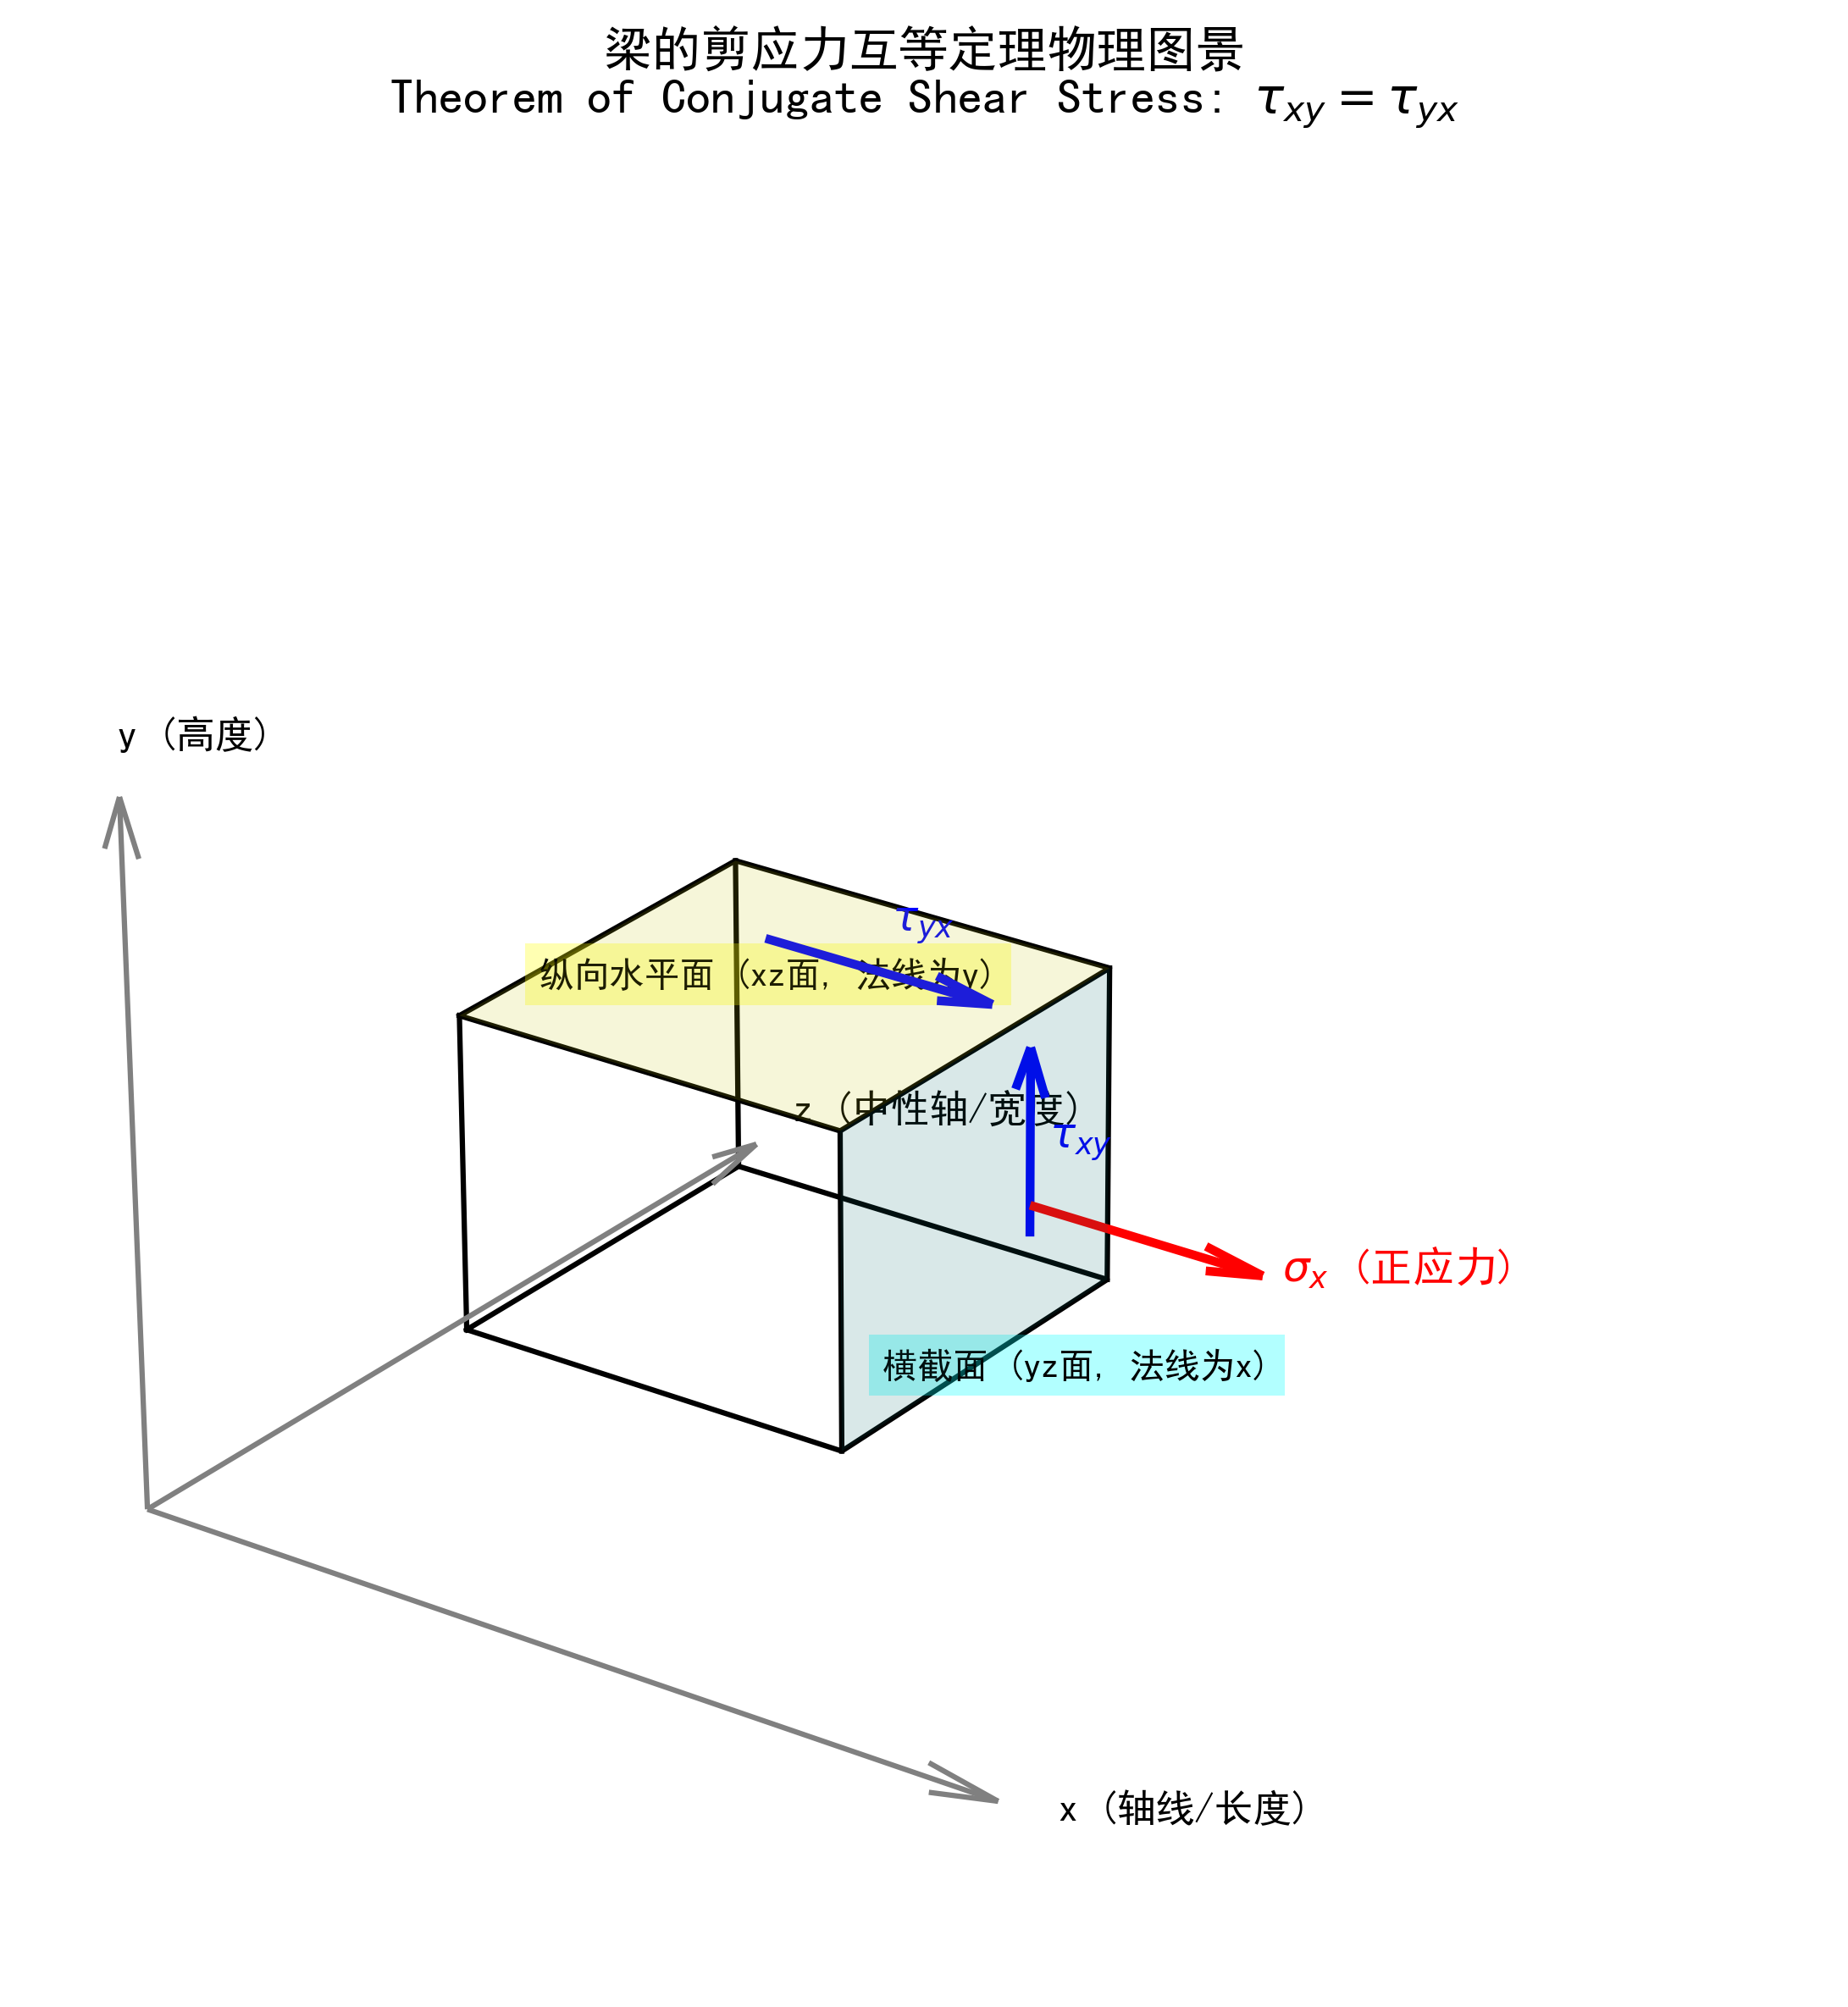
\includegraphics[width=0.42\textwidth]{shear_conjugate.png}
   \end{center}}
{剪应力命名；层间滑动；剪应力互等；剪流；静矩}

\qitem{41}{悬臂梁端部挠度}
{悬臂梁端部受力，求端部挠度和转角。}
{1. \textbf{微分方程建立}：取长度为 \(L\) 的悬臂梁，自由端受集中力 \(P\)。以固定端为原点 \(x=0\)，任意截面弯矩为 \(M(x) = -P(L-x)\)。代入控制方程：
   \[ EI w''(x) = -M(x) = P(L-x) \]
2. \textbf{二次积分求解}：
   - 积分一次求转角：\(EI w'(x) = PLx - \frac{1}{2}Px^2 + C\)。由固定端边界条件 \(w'(0) = 0 \implies C = 0\)。
   - 积分二次求挠度：\(EI w(x) = \frac{1}{2}PLx^2 - \frac{1}{6}Px^3 + D\)。由固定端边界条件 \(w(0) = 0 \implies D = 0\)。\\
3. \textbf{自由端端部最大变形（物理结果）}：将 \(x = L\) 代入：
   - 自由端最大转角：\(\theta_{\max} = w'(L) = \frac{P L^2}{2 EI}\)。
   - 自由端最大挠度：\(w_{\max} = w(L) = \frac{P L^3}{3 EI}\)。}
{边界条件；积分法；挠度}

\qitem{42}{简支梁中点挠度}
{简支梁中点受力，求中点挠度。}
{1. \textbf{对称简化与弯矩表达}：等截面简支梁（跨度 \(L\)）在中点受集中力 \(P\)。由于对称性，只需分析左半段 \(x \in [0, L/2]\)。支座反力为 \(P/2\)，左半段弯矩方程为 \(M(x) = \frac{P}{2}x\)。\\
2. \textbf{边界条件与积分}：代入梁挠曲微分方程并积分：
   \[ EI w''(x) = -M(x) = -\frac{P}{2}x \]
   - 积分一次：\(EI w'(x) = -\frac{P}{4}x^2 + C_1\)。由于对称性，中点处切线水平，转角为零：\(w'(L/2) = 0 \implies C_1 = \frac{P L^2}{16}\)。
   - 积分二次：\(EI w(x) = -\frac{P}{12}x^3 + \frac{P L^2}{16}x + C_2\)。由于左支座无位移：\(w(0) = 0 \implies C_2 = 0\)。\\
3. \textbf{中点最大挠度结果}：将中点 \(x = L/2\) 代入挠度方程得：
   \[ w_{\max} = w(L/2) = \frac{P L^3}{48 EI} \]}
{对称；分段积分；中点挠度}

\qitem{43}{弹簧支座梁}
{一根抗弯刚度为 \(EI\)、长度为 \(L\) 的梁一端由刚度为 \(k\) 的弹簧支承，中点受集中荷载 \(P\)。试用三方面分析法求弹簧的支座反力 \(R\)。}
{1. \textbf{几何变形协调}：支座处梁的向下挠度 \(w_B\) 必须等于弹簧的缩短量 \(\delta_s\)，即：\(w_B = \delta_s = \frac{R}{k}\)（\(R\) 为弹簧向上的反力）。\\
2. \textbf{物理本构关系}：利用叠加法或图乘法，梁在端部 \(B\) 处的实际位移为集中力 \(P\) 与反力 \(R\) 共同作用的结果：\(w_B = w_B^{(P)} - w_B^{(R)} = \frac{5PL^3}{48EI} - \frac{RL^3}{3EI}\)。\\
3. \textbf{静力平衡关系}：列出整体和截面的力的平衡方程，通过联立协调条件与本构关系求解未知力：
   \(\frac{5PL^3}{48EI} - \frac{RL^3}{3EI} = \frac{R}{k} \implies R = \frac{5PL^3}{48EI \cdot (\frac{1}{k} + \frac{L^3}{3EI})}\)。}
{弹簧协调；静不定；变形叠加；弹性反力}

\qitem{44}{支座沉降梁}
{连续梁某支座发生沉降，求多余反力。}
{1. \textbf{选择基本静定系}：将多余支座约束拆除，代之以未知的多余支反力 \(X_1\)，将超静定梁转化为基本静定梁。\\
2. \textbf{位移协调方程（几何关系）}：超静定梁在沉降支座处的实际挠度必须等于已知的支座沉降量 \(\Delta\)。在基本静定系上，该处的位移是由外荷载与多余反力 \(X_1\) 共同作用的结果：\(\Delta_1^{(P)} + X_1 \delta_{11} = \Delta\)。\\
3. \textbf{物理关系求解}：利用图乘法或单位载荷法求出基本静定梁在外荷载下的自由位移 \(\Delta_1^{(P)}\) 以及单位力作用下的柔度系数 \(\delta_{11}\)。\\
4. \textbf{联立求反力}：将柔度系数代回位移协调方程中，直接解出多余反力：
   \[ X_1 = \frac{\Delta - \Delta_1^{(P)}}{\delta_{11}} \]
   再由静力平衡绘制受支座沉降影响的弯矩图。}
{支座沉降；柔度；协调}

\qitem{45}{单位载荷求相对位移}
{求桁架或梁两点相对位移。}
{1. \textbf{虚拟状态的构筑}：为了求出结构上 \(A, B\) 两点沿其连线方向的相对位移 \(\Delta_{\text{rel}}\)，必须在虚拟状态下的 \(A, B\) 两点处，沿连线方向施加一对大小相等、方向相反的单位对径力 \(\bar{P} = 1\)。\\
2. \textbf{内力计算与叠加（平衡）}：
   - 真实状态：在实际外载荷作用下，计算各构件的真实内力（如弯矩 \(M(x)\)、轴力 \(N_i\)）。
   - 虚拟状态：在仅有一对单位力作用下，计算虚拟内力（如弯矩 \(\bar{M}(x)\)、轴力 \(\bar{N}_i\)）。\\
3. \textbf{虚功方程求解（物理）}：根据虚功原理，单位对径力作的外功为 \(1 \cdot \Delta_{\text{rel}}\)，等于系统的内应变能增量。计算积分或求和：
   \[ \Delta_{\text{rel}} = \sum \frac{N_i \bar{N}_i L_i}{E_i A_i} + \int_L \frac{M(x) \bar{M}(x)}{EI} \mathrm{d}x \]
   所得结果的正负号反映了相对位移是相互靠近还是相互远离。}
{相对位移；单位力；真实内力；虚内力}

\qitem{46}{卡氏定理求转角}
{用卡氏第二定理求梁某截面转角。}
{1. \textbf{引入虚拟力偶（共轭性）}：要在某截面求转角 \(\theta\)，必须在该截面上施加一个沿目标方向的虚拟力偶矩 \(M_0\)。如果该截面上已经存在真实集中力偶，则直接将其设为独立自变量。\\
2. \textbf{建立含自变量的弯矩函数}：在结构中计算含有虚拟力偶矩 \(M_0\) 的任意截面弯矩方程 \(M(x, M_0)\)。\\
3. \textbf{应用偏导求转角（卡氏第二定理）}：对结构总应变能求偏导。在求导时，可以直接将微分与积分号交换以简化计算：
   \[ \theta = \frac{\partial U}{\partial M_0} = \int_L \frac{M(x, M_0)}{EI} \frac{\partial M(x, M_0)}{\partial M_0} \mathrm{d}x \]
4. \textbf{代回真实状态}：在求导完成后，令虚拟力偶 \(M_0 = 0\)（若原本无此载荷），积分计算出真实的转角数值。}
{虚力偶；偏导；共轭位移}

\qitem{47}{压杆稳定校核}
{矩形截面压杆两端铰支，给定长度和载荷，判断是否安全。}
{1. \textbf{计算弱轴回转半径（几何）}：对非对称截面，压杆总是沿截面惯性矩最小的\textbf{弱轴}方向弯曲失稳。计算最小惯性半径：\(i_{\min} = \sqrt{I_{\min} / A}\)。根据边界约束确定长度系数 \(\mu\)，求出压杆的最大长细比：\(\lambda_{\max} = \frac{\mu L}{i_{\min}}\)。\\
2. \textbf{公式适用性判定（物理）}：
   - 若 \(\lambda_{\max} \ge \lambda_p\)（大柔度压杆，线弹性范围），使用\textbf{欧拉公式}计算临界应力：\(\sigma_{cr} = \frac{\pi^2 E}{\lambda^2}\)。
   - 若 \(\lambda_0 < \lambda_{\max} < \lambda_p\)（中柔度压杆，弹塑性范围），使用\textbf{经验公式}：\(\sigma_{cr} = a - b \lambda\)。
   - 若 \(\lambda_{\max} \le \lambda_0\)（小柔度短粗杆），发生静强度屈服失效，临界应力为材料屈服极限：\(\sigma_{cr} = \sigma_s\)。\\
3. \textbf{稳定安全校核（平衡与设计）}：工作压力为 \(P\)。稳定安全因数校核判据为：\(F_s = \frac{\sigma_{cr} A}{P} \ge [F_s]\)。}
{弱轴；长细比；临界载荷}

\qitem{48}{组合梁换算截面}
{双层材料组合梁（钢层弹性模量 \(E_s\)，铝层弹性模量 \(E_a\)，且宽为 \(b\)、高分别为 \(h_s, h_a\)）受弯矩 \(M\)，试用换算截面法求其最大应力。}
{1. \textbf{几何变形协调}：由于钢层和铝层完全粘合，各部分保持平截面，弯曲曲率 \(\kappa\) 相同，应变随高度呈线性分布：\(\varepsilon(y) = \kappa y\)。\\
2. \textbf{物理本构（应力转换）}：各层正应力为 \(\sigma_s = E_s \kappa y\)，\(\sigma_a = E_a \kappa y\)。两层应力之比为弹性模量比：\(\sigma_s / \sigma_a = E_s / E_a = n\)。\\
3. \textbf{截面换算与平衡}：将铝层换算为等效钢层，其等效宽度乘以 \(n\) 倍，即 \(b_a' = n b_a = \frac{E_a}{E_s} b\)。计算换算后单材料截面的形心位置（确定中性轴）和惯性矩 \(I_{eq}\)。\\
4. \textbf{应力求解}：等效截面的应力为 \(\sigma_s = \frac{M y}{I_{eq}}\)，铝层的实际应力需乘上换算比例：\(\sigma_a = \frac{1}{n} \sigma_s = \frac{E_a}{E_s} \frac{M y}{I_{eq}}\)。}
{平截面假设；换算宽度；模量比；等效惯性矩}

\qitem{49}{疲劳应力循环}
{给出 \(\sigma_{\max},\sigma_{\min}\)，求应力幅、平均应力和循环特征。}
{1. \textbf{最大最小应力确定（静力与本构）}：由工作载荷的循环波动范围，通过材料力学公式求出危险点处交变应力的最大值 \(\sigma_{\max}\) 和最小值 \(\sigma_{\min}\)。\\
2. \textbf{应力环特征物理量计算}：
   - \textbf{平均应力}：\(\sigma_m = \frac{\sigma_{\max} + \sigma_{\min}}{2}\)。
   - \textbf{应力幅}：\(\sigma_a = \frac{\sigma_{\max} - \sigma_{\min}}{2}\)。
   - \textbf{循环特征（应力比）}：\(r = \frac{\sigma_{\min}}{\sigma_{\max}}\)。\\
3. \textbf{典型循环类型分类}：
   - 对称循环：\(r = -1\)，此时平均应力 \(\sigma_m = 0\)（如旋转弯曲轴表面的应力状态）。
   - 脉动循环：\(r = 0\)，此时最小应力为 0，\(\sigma_m = \sigma_a\)。
   - 恒定应力（静应力）：\(r = 1\)，无交变波动。}
{应力幅；平均应力；应力比}

\qitem{50}{冲击梁动荷载}
{重物从高度 \(h\) 落到弹性梁上，求最大动应力。}
{1. \textbf{静挠度计算（物理第一步）}：计算重物加载位置在静止放置时的\textbf{最大静挠度} \(\Delta_{st}\)（可套用梁的静位移公式）。\\
2. \textbf{动载荷系数确定（能量守恒）}：重物自高度 \(h\) 自由下落冲击梁。重力势能转化为梁的应变能，由动能定理和守恒定律导出动载系数：
   \[ K_d = 1 + \sqrt{1 + \frac{2h}{\Delta_{st}}} \]
   若为突然释放（无落高，\(h=0\)），则 \(K_d = 2\)。\\
3. \textbf{最大动应力与动挠度校核（平衡与叠加）}：
   - 最大动挠度：\(w_{d} = K_d \cdot \Delta_{st}\)。
   - 最大动应力：\(\sigma_{d} = K_d \cdot \sigma_{st}\)（\(\sigma_{st}\) 为将重物静止放置于梁上时产生的最大静弯曲正应力）。
   强度要求 \(\sigma_d \le [\sigma]\)。}
{冲击；静挠度；动载系数}

\chap{三、对称性与微元法 20 份}

\qitem{51}{对称梁反力}
{对称简支梁受对称荷载，说明为什么两支座反力相等。}
{1. \textbf{结构与荷载的对称性定义}：如果一个梁的几何形状、跨度、支座约束位置关于跨中轴对称，且其承受的外力载荷大小和位置也关于跨中轴对称。\\
2. \textbf{反力对称性推导}：由于边界和载荷完全对称，左右两个支座的反力必然满足完全相等的物理约束：\(R_A = R_B\)。\\
3. \textbf{静力平衡应用}：列竖向平衡方程 \(\sum F_y = 0 \implies R_A + R_B = P_{\text{total}} \implies 2 R_A = P_{\text{total}}\)。由此直接解得每个支座反力等于总竖向荷载的一半：\(R_A = R_B = \frac{1}{2} P_{\text{total}}\)。此对称性判定在大题中无须写出力矩平衡方程，可瞬间化简。}
{结构对称；荷载对称；反力对称}

\qitem{52}{对称截面转角为零}
{对称梁在对称荷载下，证明跨中转角为零。}
{1. \textbf{变形曲线的对称性特征}：在对称结构和对称荷载作用下，梁发生弯曲变形后，其挠度曲线 \(w(x)\) 必然也关于跨中轴对称。\\
2. \textbf{数学斜率（奇函数）分析}：若挠曲线关于原点（跨中 \(x=0\) 处）对称，则挠度函数为偶函数：\(w(x) = w(-x)\)。对其求导得到斜率（转角）函数为：\(w'(x) = -w'(-x)\)，即转角函数 \(\theta(x) = w'(x)\) 必然是奇函数。\\
3. \textbf{跨中转角零值结论}：根据奇函数在原点连续的数学定理，自变量为零处对应的奇函数值必为零：\(\theta(0) = 0\)。因此，对称弯曲梁的跨中截面在变形后其切线仍保持水平，无转角。这在图乘法或积分法中是一个极其重要的边界条件。}
{挠曲线对称；斜率；跨中}

\qitem{53}{反对称荷载}
{说明反对称荷载下对称截面位移/内力的特点。}
{1. \textbf{荷载与变形奇偶性定义}：结构关于跨中对称，但荷载关于跨中反对称（例如左半跨受向下均布力 \(q\)，右半跨受向上均布力 \(q\)）。此时，变形后的挠曲线 \(w(x)\) 必须是关于中点的奇函数，即满足：\(w(x) = -w(-x)\)。\\
2. \textbf{对称轴面上零量判定}：\\
   - \textbf{位移零值}：根据奇函数定义，跨中对称截面处的挠度（垂直位移）必须为零：\(w(0) = 0\)。\\
   - \textbf{弯矩零值}：由于弯矩与挠曲线的二阶导数成正比（奇函数求导两次仍为奇函数），跨中对称面上的弯矩必然为零：\(M(0) = 0\)。\\
3. \textbf{内力与反力简化的应用}：反对称弯曲时，两侧对称反力大小相等、方向相反：\(R_A = -R_B\)。在力法中，跨中截面可直接简化为铰接点（弯矩为 0）或者剪切铰。}
{反对称；奇偶性；边界简化}

\qitem{54}{圆环对称分析与弯矩图}
{圆环受一对垂直对径集中力 \(F_P\)，请画出其简化模型，并说明如何利用结构和载荷的对称性选择合理的切开位置、分析切口截面上的内力并画出弯矩图。}
{1. \textbf{对称轴分析}：圆环在几何形状、边界约束及垂直对径力下具有垂直对称轴 \(AB\) 和水平对称轴 \(CD\)（见下方图）。\\
2. \textbf{切口选择与零内力判定}：取水平截面 \(C, D\) 切开。根据对称性，反对称剪力 \(V_0 = 0\)。由垂直方向静力平衡，对称轴力 \(F_{N0} = F_P/2\)（拉力）。结构简化为仅含唯一未知对称冗余弯矩 \(M_0\) 的超静定系统。\\
3. \textbf{弯矩分布规律}：最大弯矩发生在加载点 \(A, B\) 处。
   \begin{center}
     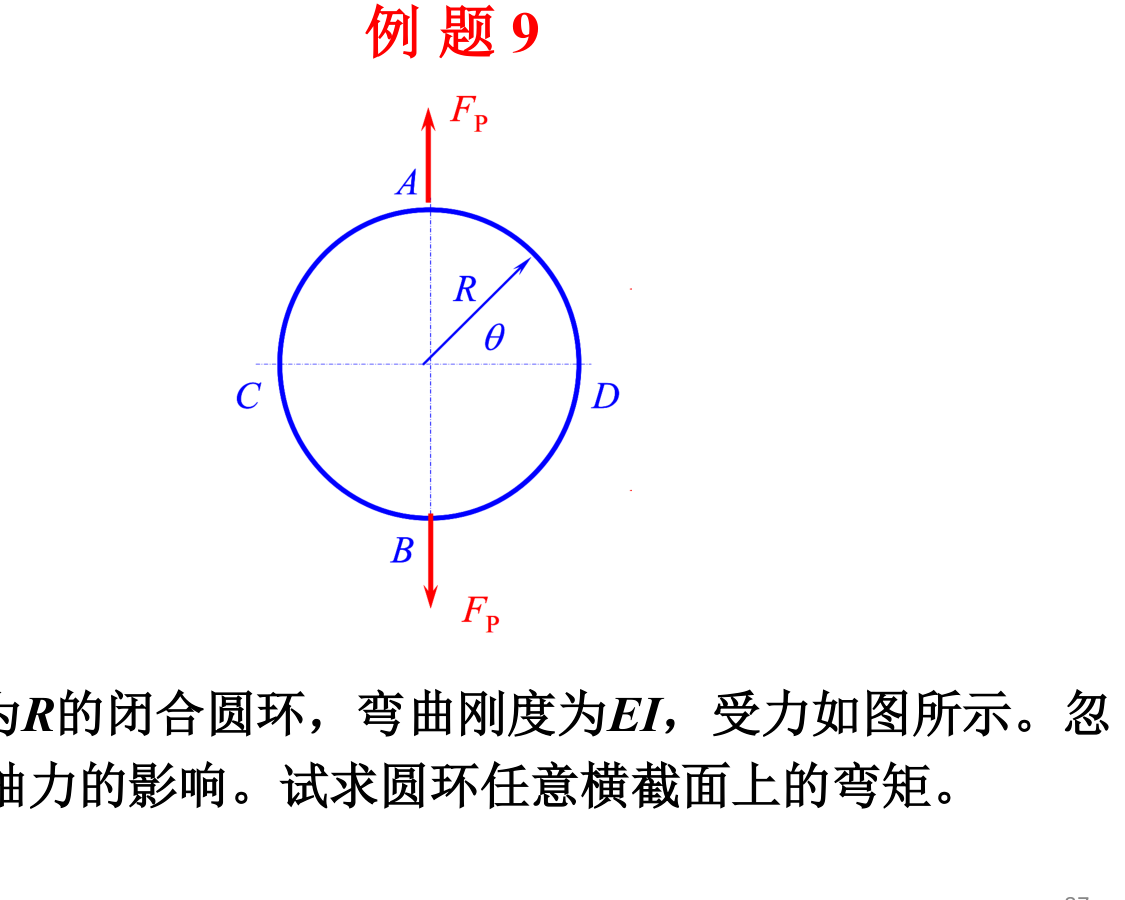
\includegraphics[width=0.42\textwidth]{ring_problem.png} \hfill
     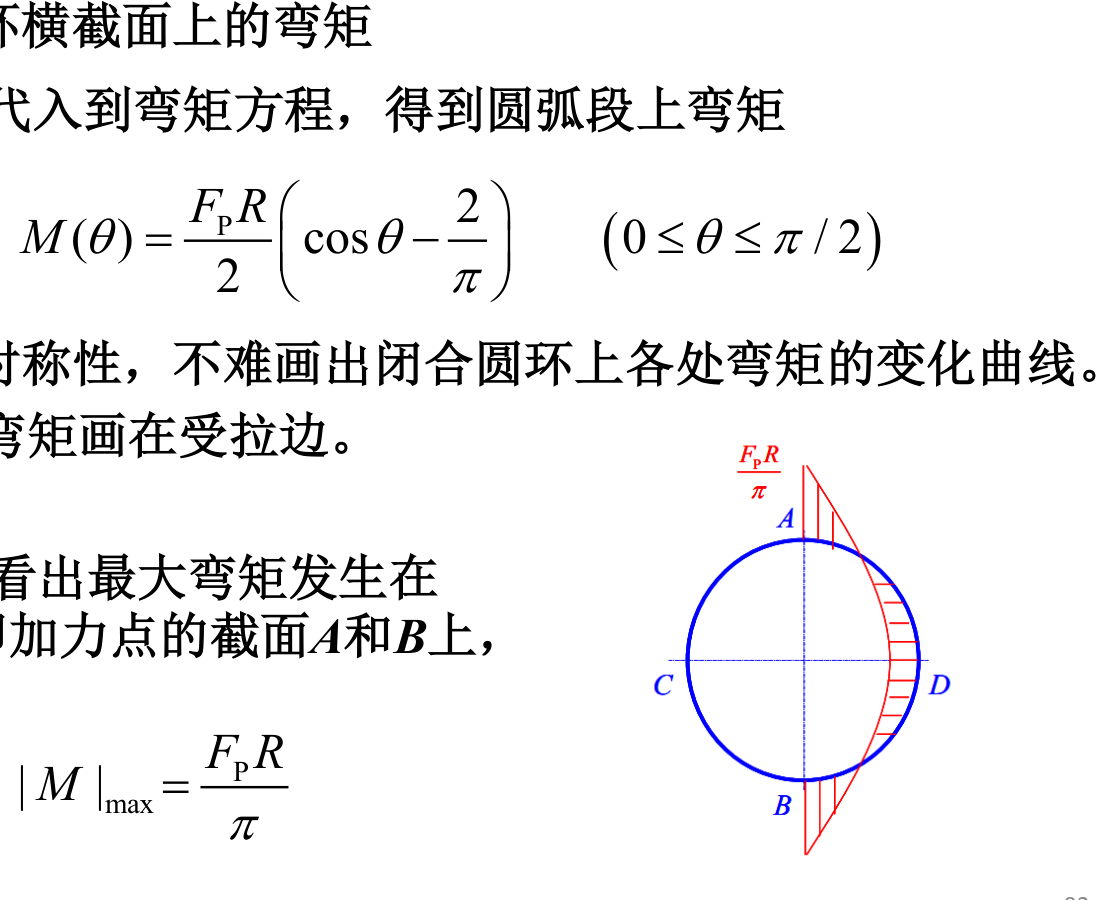
\includegraphics[width=0.42\textwidth]{ring_moment.png}
   \end{center}}
{对称轴；剪力为零；轴力平衡；冗余弯矩；弯矩图}

\qitem{55}{超静定圆环求解}
{对于受垂直对径力 \(F_P\) 的闭合圆环，说明如何建立变形协调方程求解冗余弯矩 \(M_0\)，写出任意截面的弯矩函数表达式，并求极值弯矩（弯矩分布图见上题图）。}
{1. \textbf{建立弯矩函数}：以水平对称截面 \(C\) 为起点（\(\theta=0\)），截取任意角度 \(\theta\)（\(0 \le \theta \le \pi/2\)）的圆弧段，其横截面上的弯矩为：
   \[ M(\theta) = M_0 - F_{N0} R (1 - \cos\theta) = M_0 - \frac{F_P}{2} R (1 - \cos\theta) \]
2. \textbf{变形协调方程（卡氏第二定理）}：由于对称性，水平切口 \(C\) 处的两侧截面没有相对转角 \(\theta_{rel} = 0\)。对 4 个 \(\pi/2\) 圆弧段的总弯曲应变能 \(U\) 应用卡氏第二定理：
   \[ \frac{\partial U}{\partial M_0} = 4 \int_0^{\pi/2} \frac{M(\theta) R}{EI} \frac{\partial M(\theta)}{\partial M_0} \mathrm{d}\theta = 0 \]
   由于 \(\frac{\partial M(\theta)}{\partial M_0} = 1\)，代入得：
   \[ \int_0^{\pi/2} \left[ M_0 - \frac{F_P}{2} R (1 - \cos\theta) \right] \mathrm{d}\theta = 0 \implies M_0 \frac{\pi}{2} - \frac{F_P R}{2}\left(\frac{\pi}{2} - 1\right) = 0 \]
   解得水平对称面处的弯矩：
   \[ M_0 = \frac{F_P R}{2} \left( 1 - \frac{2}{\pi} \right) \approx 0.182 F_P R \]
3. \textbf{任意截面弯矩与极值}：将 \(M_0\) 代回得弯矩函数为：
   \[ M(\theta) = F_P R \left( \frac{\cos\theta}{2} - \frac{1}{\pi} \right) \quad \left(0 \le \theta \le \frac{\pi}{2}\right) \]
   \begin{itemize}
     \item 在 \(\theta = 0\)（水平侧面处）：\(M(0) = M_0 \approx 0.182 F_P R\)（外侧受拉）。
     \item 在 \(\theta = \pi/2\)（垂直顶端加载点处）：\(M(\pi/2) = -F_P R/\pi \approx -0.318 F_P R\)（内侧受拉）。
     \item 最大弯矩绝对值为 \(\frac{F_P R}{\pi}\)（发生在加载点 \(A, B\) 处）。
   \end{itemize}}
{协调方程；卡氏定理；对称性；弯矩函数；极值弯矩}


\qitem{56}{梁微元平衡}
{建立梁微元体平衡方程，推导弯矩、剪力与分布荷载之间的微分关系：\(\frac{dV}{dx}=-q(x)\)，\(\frac{dM}{dx}=V(x)\)。}
{1. \textbf{微元体分析}：取出长度为 \(dx\) 的梁微段，其左侧剪力为 \(V\)、弯矩为 \(M\)；右侧剪力为 \(V+dV\)、弯矩为 \(M+dM\)；表面受向下分布载荷 \(q(x)\)。\\
2. \textbf{竖向力平衡}：
   \(\sum F_y = 0 \implies V - (V+dV) - q(x)dx = 0 \implies \frac{dV}{dx} = -q(x)\)。\\
3. \textbf{绕右端点力矩平衡}：
   \(\sum M_{right} = 0 \implies (M+dM) - M - V \cdot dx - q(x)dx \cdot \frac{dx}{2} = 0\)。\\
4. \textbf{忽略二阶无穷小} \(q(x)\frac{(dx)^2}{2}\) 得：
   \(dM = V \cdot dx \implies \frac{dM}{dx} = V(x)\)。}
{竖向平衡；力矩平衡；高阶小量；剪力弯矩微分关系}

\qitem{57}{轴向杆微分方程}
{对有分布轴向载荷的杆，用微元平衡建立 \(N(x)\) 方程。}
{1. \textbf{微元体分析}：取长为 \(dx\) 的杆段，左端受轴力 \(N(x)\)，右端受轴力 \(N+dN\)，表面受轴向分布载荷 \(q_x(x)\)（向右为正）。\\
2. \textbf{平衡方程}：列轴向平衡得：\(\sum F_x = 0 \implies (N+dN) - N + q_x(x)dx = 0\)。\\
3. \textbf{微分关系}：消去并化简得到 \(\frac{dN}{dx} + q_x(x) = 0\)，即轴力变化率等于负的分布轴向载荷。}
{轴向分布载荷；微段；内力变化率}

\qitem{58}{圆轴扭转微元}
{对有分布扭矩的圆轴，用微元法建立扭矩微分方程。}
{1. \textbf{微元体分析}：取长为 \(dx\) 的圆轴段，左端受扭矩 \(T(x)\)（右手螺旋指向外为正），右端受扭矩 \(T+dT\)，外表面受分布扭矩 \(m(x)\)。\\
2. \textbf{力矩平衡}：对轴线列矩平衡：\(\sum M_x = 0 \implies (T+dT) - T + m(x)dx = 0\)。\\
3. \textbf{微分关系}：化简得到 \(\frac{dT}{dx} + m(x) = 0\)，即扭矩图的斜率等于负的分布扭矩强度。}
{分布扭矩；扭矩图；微元平衡}

\qitem{59}{开口薄壁截面的剪应力流与剪切中心（弯扭解耦）}
{用微元平衡解释薄壁梁中剪应力流的概念，说明为什么非对称开口薄壁截面梁（如槽钢）在仅受横向力作用时会自发扭转，并阐明“剪切中心”的定义及如何利用力矩平衡确定其位置。}
{1. \textbf{剪应力流微元平衡}：\\
   薄壁截面中，壁厚 \(t\) 极小，剪应力 \(\tau\) 沿中面切向分布。定义剪应力流为单位长度上的切向剪力：\(q = \tau t\)。沿薄壁轴线截取长 \(\mathrm{d}x\)、切向宽 \(\mathrm{d}s\) 的板条微元。由轴向正应力差引起的纵向力平衡方程为：
   \[ \frac{\partial q}{\partial s} + t \frac{\partial \sigma}{\partial x} = 0 \implies q(s) = q_0 - \int_0^s t \frac{\partial \sigma}{\partial x} \mathrm{d}s \]
   这说明正应力沿轴向的变化直接激发起截面上的剪流分布。\\
2. \textbf{自发扭转的物理成因}：\\
   - 在开口非对称截面（如槽钢，开口向右）中，剪力 \(V\) 在腹板和翼缘中激发起顺着壁中线的弯曲剪流。
   - 翼缘中的水平剪流大小相等、方向相反，形成一个水平力偶矩 \(T_{\text{flow}} = H \cdot b\)（其中 \(H\) 为翼缘剪力合力，\(b\) 为槽钢高度）。此力偶矩在截面上会产生绕轴线的扭转作用。
   - 即使外力没有施加外扭矩，只要外力作用在截面形心上，外力对该剪流合力就会产生力矩不平衡，从而导致梁在发生弯曲时\textbf{自发发生扭转}。\\
3. \textbf{剪切中心与力矩平衡位置确定}：\\
   - \textbf{定义}：截面上存在一个特殊点，当横向外力作用线通过该点时，外力对该点产生的力矩与截面剪应力流的合力矩刚好平衡，梁\textbf{只发生弯曲、不发生扭转}。这个点称为\textbf{剪切中心}（Shear Center）。
   - \textbf{计算位置（力矩平衡）}：以槽钢为例，翼缘水平力为 \(H\)，腹板竖向力合力等于外剪力 \(V\)。设外力 \(V\) 作用在腹板左侧距离为 \(e\) 处（即剪切中心）。对腹板与中轴交点列矩平衡：
     \[ V \cdot e = H \cdot b \implies e = \frac{H b}{V} \]
     此式决定了剪切中心偏离形心的位置。剪切中心是\textbf{截面的固有几何特性}，与外力大小无关。双对称截面的剪切中心与形心重合；单对称截面的剪力中心必在对称轴上。}
{剪流微元；自发扭转；力偶矩；剪切中心；只弯不扭；几何特性}

\qitem{60}{压杆微分方程}
{用微小扰动法建立压杆屈曲微分方程。}
{1. \textbf{挠度与弯矩}：设两端铰支压杆受轴向压力 \(P\)，挠曲线为 \(w(x)\)。截面弯矩为 \(M(x) = -P w(x)\)。\\
2. \textbf{微分方程}：代入挠曲线近似微分方程：\(EI \frac{d^2w}{dx^2} = -P w \implies \frac{d^2w}{dx^2} + k^2 w = 0\)（其中 \(k^2 = \frac{P}{EI}\)）。\\
3. \textbf{通解与边界条件}：通解为 \(w(x) = A\sin(kx) + B\cos(kx)\)。代入边界条件 \(w(0)=0 \implies B=0\)；\(w(L)=0 \implies A\sin(kL)=0\)。\\
4. \textbf{临界载荷}：若有非零屈曲解（\(A \ne 0\)），必有 \(\sin(kL)=0 \implies kL=\pi\)（一阶失稳），解得 \(P_{cr} = \frac{\pi^2 EI}{L^2}\)（欧拉公式）。}
{微小扰动；非零解；屈曲}

\qitem{61}{弯曲中性轴对称}
{对称截面纯弯曲时，利用对称性判断中性轴位置。}
{1. \textbf{形心判定}：纯弯曲梁截面上轴力 \(N = \int_A \sigma \mathrm{d}A = E \kappa \int_A y \mathrm{d}A = 0\)，说明中性轴必通过截面几何形心。\\
2. \textbf{方向判定}：当横截面关于某轴（如 \(y\) 轴）对称且弯矩绕另一轴（如 \(z\) 轴）作用时，弯曲面不发生斜弯曲，中性轴（\(z\) 轴）垂直于对称轴且通过形心。}
{对称轴；形心；无轴力}

\qitem{62}{组合截面对称简化}
{组合截面关于某轴对称，说明形心和主惯性轴如何简化。}
{1. \textbf{形心位置}：若截面关于某轴（如 \(y\) 轴）对称，该轴一侧的静矩与另一侧抵消，总静矩 \(S_z=0\)，形心必在对称轴上。\\
2. \textbf{主惯性轴}：对称轴与垂直于它的任一轴（如 \(z\) 轴）的惯性积为：\(I_{yz} = \int_A y z \mathrm{d}A = 0\)（对称点积相消）。\\
3. \textbf{结论}：对称轴空间形心主轴，对应的惯性积为零，极大简化了惯性矩计算。}
{对称轴；主轴；惯性积}

\qitem{63}{莫尔圆对称性}
{解释莫尔圆中相互垂直截面为什么对应圆上相差 \(180^\circ\) 的两点。}
{1. \textbf{物理关系}：在应力变换公式中，截面法线旋转 \(\theta\) 角时，正应力和剪应力的变换公式中均含有双倍角 \(2\theta\)。\\
2. \textbf{圆上对应}：物理截面上互为垂直的两个面（法线相差 \(\theta = 90^\circ\)），在应力莫尔圆上对应的点相差的角度为 \(2\theta = 180^\circ\)，正好是直径的两个端点。\\
3. \textbf{物理表现}：这证明了垂直截面上正应力之和为常数（\(\sigma_x + \sigma_y = \text{const}\)），且剪应力大小相等、方向相反（\(\tau_{xy} = -\tau_{yx}\)）。}
{二倍角；垂直截面；莫尔圆}

\qitem{64}{圆轴截面对称性}
{利用圆截面对称性说明 \(I_y=I_z=I_p/2\)。}
{1. \textbf{直径等价性}：圆截面具有完全的旋转轴对称性，通过圆心的任意两条正交直径（\(y, z\) 轴）完全等价，故弯曲惯性矩相等：\(I_y = I_z\)。\\
2. \textbf{极惯性矩关系}：根据定义，极惯性矩 \(I_p = \int_A \rho^2 \mathrm{d}A = \int_A (y^2+z^2)\mathrm{d}A = I_z + I_y\)。\\
3. \textbf{公式确定}：联立得 \(I_y = I_z = \frac{1}{2} I_p\)。对半径为 \(R\) 的圆，\(I_p = \frac{\pi R^4}{2}\)，故 \(I_y = I_z = \frac{\pi R^4}{4}\)。}
{圆对称；极惯性矩；正交轴}

\qitem{65}{移动荷载对称}
{简支梁上移动集中力何时产生最大弯矩，如何用对称性判断。}
{1. \textbf{移动荷载极值原理}：在工程结构（如桥梁梁）上，当一个或一组集中力在跨间任意移动时，梁内危险截面的最大弯矩必定发生在移动集中力所在的截面处。\\
2. \textbf{对称支座下的最不利位置}：对两端对称铰支的简支梁（跨度 \(L\)），如果只有一个移动力 \(F_P\)，当力移动到位置 \(x\) 处时，受力截面的弯矩为 \(M(x) = F_P \cdot \frac{x(L-x)}{L}\)。\\
3. \textbf{跨中极值结论}：由于二次函数 \(y = x(L-x)\) 的对称轴和顶点在跨中 \(x = L/2\) 处，当移动荷载正好行驶到梁的跨中点时，梁的全局最大弯矩达到峰值：\(M_{\max} = \frac{F_P L}{4}\)。}
{影响线；对称；最大弯矩}

\qitem{66}{反力影响线微元思想}
{说明影响线为什么可以看成单位移动荷载引起的响应函数。}
{1. \textbf{影响线物理定义}：影响线是描述当一个\textbf{单位移动集中力 \(\bar{P} = 1\)} 沿结构移动时，结构上某一特定截面的内力（如剪力、弯矩）或支座反力随荷载作用位置 \(x\) 变化的响应函数曲线。\\
2. \textbf{微元移动分析思想}：将移动荷载的位置坐标 \(x\) 作为自变量。单位力每前移一微元 \(\mathrm{d}x\)，对应的支座反力会产生微小增量 \(\mathrm{d}R\)。影响线上的纵坐标值直接对应着力作用在此位置时反力的大小。\\
3. \textbf{实际多载荷快速计算}：一旦绘出影响线函数 \(Y(x)\)，当有一组任意大小的移动力系 \(F_i\) 作用时，该反力的总响应无需重新做静力平衡，可由各力乘以对应影响线纵坐标的乘积直接叠加得到：\(R = \sum F_i Y(x_i)\)。}
{单位移动荷载；响应函数；影响线}

\qitem{67}{曲杆微元内力}
{对平面曲杆微元说明内力包含轴力、剪力和弯矩，且方向随切线转动。}
{1. \textbf{曲率引起的内力方向转动}：直杆的内力方向在全局坐标系下是恒定的。但对于平面曲杆，由于轴线本身是弯曲的，在截取长 \(\mathrm{d}s = R\mathrm{d}\theta\) 的弧段微元时，微元左、右两侧横截面的法线（切线）方向存在夹角 \(\mathrm{d}\theta\)。\\
2. \textbf{局部坐标系与内力定义}：在曲杆的每个横截面上，建立局部“切向-法向（纵向-径向）”坐标系。
   - 轴力 \(N\) 沿切线方向，导致曲杆伸缩。
   - 剪力 \(V\) 沿法线方向，导致层间错动。
   - 弯矩 \(M\) 绕主轴，导致曲率改变。\\
3. \textbf{微元平衡方程建立}：列出局部切向和法向的力的平衡时，必须将左右两侧截面内力乘以三角函数进行投影（由于夹角 \(\mathrm{d}\theta\) 的存在，左侧轴力会部分投影到右侧剪力方向）。微分平衡方程中会显式地包含曲率半径 \(R\) 的项。}
{曲杆；局部坐标；曲率}

\qitem{68}{圆环弯矩函数}
{对于半径为 \(R\) 的曲杆或圆环，详细说明如何使用截面法以圆心角 \(\theta\) 为变量建立任意截面的弯矩函数 \(M(\theta)\)，并指出外力对截面形心力矩的力臂计算规律。}
{1. \textbf{截开隔离体}：从参考截面（通常选择已知内力的对称截面或自由端）处截开，以圆心角 \(\theta\) 定位任意待求截面。\\
2. \textbf{确定力臂规律}：设某外力（或已知内力）作用在圆心角 \(\phi\) 处，待求截面在圆心角 \(\theta\) 处。
   \begin{itemize}
     \item \textbf{径向外力 \(F_r\) 对截面的力臂}：力作用线至待求截面形心的垂直距离为 \(d = R \sin(\theta - \phi)\)。
     \item \textbf{切向外力 \(F_t\) 对截面的力臂}：力矩臂为 \(d = R [1 - \cos(\theta - \phi)]\)。
     \item \textbf{对径集中力 \(F_P\) 对半圆弧截面的力臂}：若参考端为水平对称面（\(\theta=0\)），位于 \(\theta=\pi/2\) 的力 \(F_P/2\) 对截面 \(\theta\) 的力臂为 \(d = R(1 - \cos\theta)\)（力作用线垂直）。
   \end{itemize}
3. \textbf{建立力矩平衡}：对待求截面形心列力矩平衡方程 \(\sum M_{centroid} = 0\)，即可直接解出 \(M(\theta)\)。在画弯矩图或列方程时，注意内力弯矩的正负号规定必须与应变能公式中的符号保持一致。}
{截面法；圆心角；力臂投影；力矩平衡；弯矩函数}

\qitem{69}{对称性判断零量}
{列举对称面上哪些量可能为零，并说明判断规则。}
{1. \textbf{对称与反对称内力/变形分类}：\\
   - \textbf{对称量}：在跨中截面关于对称轴对称分布的量（如正应力 \(\sigma\)、弯矩 \(M\)、轴力 \(N\)、竖向位移 \(w\)）。\\
   - \textbf{反对称量}：在跨中两侧符号相反的量（如剪力 \(V\)、转角 \(\theta\)、水平位移 \(u\)）。\\
2. \textbf{对称荷载作用下}：\\
   整个结构的响应必须对称，这意味着任何反对称量在跨中对称轴截面上必须为零：
   - 剪力必为零：\(V(0) = 0\)。
   - 水平位移与转角必为零：\(u(0) = 0, \theta(0) = 0\)。\\
3. \textbf{反对称荷载作用下}：\\
   整个结构的响应必须反对称，这意味着任何对称量在跨中对称轴截面上必须为零：
   - 轴力必为零：\(N(0) = 0\)。
   - 弯矩必为零：\(M(0) = 0\)。
   - 竖向挠度必为零：\(w(0) = 0\)。}
{对称量；反对称量；零边界条件}

\qitem{70}{微元法与积分法关系}
{说明微元法建立微分方程后为什么还需要边界条件。}
{1. \textbf{微元法的物理本质（微分方程）}：微元法通过对无限小构件进行平衡分析，建立反映系统局部内力与载荷之间变化关系的微分方程（如 \(\frac{\mathrm{d}^2w}{\mathrm{d}x^2} = -\frac{M}{EI}\)）。这代表了结构内部\textbf{处处满足的局部微分约束}，但不涉及端部的具体固定形式。\\
2. \textbf{积分法的物理本质（通解求取）}：积分法是对上述局部微分方程在全局长度上进行一阶或高阶积分，以求出变形和内力的通解函数。在求积分的过程中，每积分一次都会产生一个未知的数学常数。\\
3. \textbf{边界条件与定解（约束确定）}：这些积分常数代表了系统在没有外部约束时的刚体位移自由度。只有代入具体的物理边界约束条件（如固定端的位移和转角为 0，简支端的挠度为 0）和变形连续条件，才能唯一确定这些常数。}
{局部平衡；积分常数；边界条件}

\chap{四、综合计算变式 20 份}

\qitem{71}{温度杆 + 压杆稳定}
{两根钢柱支撑刚性梁，中间铝杆加热顶紧梁。求温度应力并校核钢柱稳定。}
{1. \textbf{第一步：温度引起的不平衡变形（力学协调）}：\\
   - 计算中间铝杆受热后的自由热膨胀量：\(\Delta_T = \alpha_a \Delta T L\)。\\
   - 判断铝杆是否顶紧刚性梁：若自由膨胀量大于初始间隙 \(\delta\)，则顶紧并受压。\\
   - 建立变形协调：铝杆的实际缩短量加钢柱的弹性缩短量等于自由膨胀量扣除间隙：\(\Delta l_{Fa} + \Delta l_{Fs} = \Delta_T - \delta\)。\\
2. \textbf{第二步：内力分析（静力平衡）}：\\
   由本构关系代入变形协调方程，解出铝杆轴力 \(N_a\) 以及两根钢柱平分的分担压轴力：\(P_s = N_s = \frac{1}{2} N_a\)。\\
3. \textbf{第三步：压杆稳定校核}：\\
   - 确定钢柱的弱轴方向计算惯性矩 \(I_{\min}\) 与最大长细比 \(\lambda\)。\\
   - 利用欧拉公式计算单根钢柱的临界屈曲载荷：\(P_{cr} = \frac{\pi^2 E_s I_{\min}}{(\mu L)^2}\)。\\
   - 比较实际工作轴力 \(N_s\) 与临界力 \(P_{cr}\)，稳定安全系数为 \(F_s = P_{cr} / N_s \ge [F_s]\)。}
{温度；静不定；压杆；安全因数}

\qitem{72}{扭转 + 强度理论}
{圆轴同时承受扭矩 and 轴向拉力，求危险点主应力并按第四强度理论校核。}
{1. \textbf{截面内力与工作应力计算}：\\
   - 承受轴向拉力 \(N\) 产生的均匀拉应力：\(\sigma_x = \frac{N}{A} = \frac{4N}{\pi d^2}\)。\\
   - 承受扭矩 \(T\) 产生外表面的最大切应力：\(\tau_{xy} = \frac{T}{W_p} = \frac{16T}{\pi d^3}\)。\\
2. \textbf{危险点应力状态构筑}：\\
   圆轴表面的危险点处于平面应力状态，其中正应力分量为 \(\sigma_x\)，剪应力分量为 \(\tau_{xy}\)，横向正应力 \(\sigma_y = 0\)。\\
3. \textbf{主应力与强度准则校核}：\\
   根据第四强度理论（畸变能准则），相当应力公式化为：
   \[ \sigma_{eq4} = \sqrt{\sigma_x^2 + 3 \tau_{xy}^2} = \sqrt{\left(\frac{4N}{\pi d^2}\right)^2 + 3\left(\frac{16T}{\pi d^3}\right)^2} \]
   强度条件为 \(\sigma_{eq4} \le [\sigma]\)。}
{拉扭组合；平面应力；Mises}

\qitem{73}{梁弯曲 + 剪切}
{短粗矩形梁受集中力，要求同时校核正应力和剪应力。}
{1. \textbf{绘制剪力与弯矩内力图（平衡）}：分析外载荷，求出剪力图 \(V(x)\) 和弯矩图 \(M(x)\)。危险截面通常为弯矩最大截面（\(M_{\max}\)）和剪力最大截面（\(V_{\max}\)）。\\
2. \textbf{危险点正应力校核（物理第一步）}：\\
   在弯矩 \(M_{\max}\) 截面的最外侧边缘纤维（距离中性轴 \(y_{\max}\) 处），其正应力最大：\(\sigma_{\max} = \frac{|M_{\max}|}{W_z}\)。校核 \(\sigma_{\max} \le [\sigma]\)。\\
3. \textbf{危险点剪应力校核（物理第二步）}：\\
   在剪力 \(V_{\max}\) 截面的中性轴线处（此处静矩 \(Q\) 最大），其剪应力最大：\(\tau_{\max} = \frac{V_{\max} Q_{\max}}{I_z b}\)。对于矩形截面，简写为 \(\tau_{\max} = 1.5 \frac{V_{\max}}{A}\)。校核 \(\tau_{\max} \le [\tau]\)。}
{正应力；剪应力；危险点不同}

\qitem{74}{偏心压缩 + 核心}
{偏心压力作用于矩形截面柱，求是否出现拉应力并画应力分布。}
{1. \textbf{应力公式叠加}：偏心压缩载荷 \(P\) 作用在坐标 \((e_y, e_z)\) 处。截面上任意点 \((y, z)\) 的应力公式为：
   \[ \sigma = -\frac{P}{A} - \frac{P e_y y}{I_z} - \frac{P e_z z}{I_y} \]
2. \textbf{最不利零点应力求解}：\\
   - 确定拉应力最大（即压应力最小）的位置，通常发生在偏心载荷对角线另一侧的截面顶点。\\
   - 令该顶点的应力为 0：\(\sigma(y_{\text{corner}}, z_{\text{corner}}) = 0\)。这在几何上给出了中性轴正好切于截面边缘的临界状态。\\
3. \textbf{截面核心区域确定}：\\
   偏心距极限方程为：\(1 + \frac{A e_y y_{\text{corner}}}{I_z} + \frac{A e_z z_{\text{corner}}}{I_y} = 0\)。这在 \((e_y, e_z)\) 偏心距平面上围成一个多边形区域，称为\textbf{截面核心}。只要压力作用在此核心内，截面上就不会产生拉应力。}
{偏心距；核心；应力分布}

\qitem{75}{组合梁 + 能量法}
{完全粘合组合梁受集中力，求中点挠度。}
{1. \textbf{第一步：几何换算截面}：\\
   - 将双材料梁通过模量比 \(n = E_2 / E_1\) 换算成单一材料（如材料 1）的截面。\\
   - 求出换算后等效单材料截面的中性轴形心位置以及等效惯性矩 \(I_{eq}\)。\\
   - 确定等效弯曲刚度：\(D = E_1 I_{eq}\)。\\
2. \textbf{第二步：能量法表达建立}：\\
   - 写出梁内由外载荷产生的弯矩方程 \(M(x)\)。\\
   - 梁的总弯曲应变能表示为：\(U = \int_L \frac{M^2(x)}{2 D} \mathrm{d}x = \int_L \frac{M^2(x)}{2 E_1 I_{eq}} \mathrm{d}x\)。\\
3. \textbf{第三步：求位移（卡氏定理或单位载荷法）}：\\
   - 对集中力 \(P\) 求偏导即可直接得出组合梁的中点挠度：\(w = \frac{\partial U}{\partial P}\)。}
{换算截面；等效刚度；单位载荷}

\qitem{76}{支座沉降 + 弯矩图}
{一端固定一端支承梁，支座沉降 \(\delta\)，求多余反力并画弯矩图。}
{1. \textbf{建立超静定力法方程}：\\
   设一端固定、一端支承的超静定梁，支承端发生沉降 \(\Delta\)。选择支承反力 \(R\) 为多余冗余力。\\
2. \textbf{位移协调与本构联立}：\\
   - 自由状态（仅受外均布载荷 \(q\)）：支承端处的挠度为 \(w_q = \frac{q L^4}{8 EI}\)（向下）。\\
   - 冗余力作用（仅受向上的反力 \(R\)）：支承端处的挠度为 \(w_R = \frac{R L^3}{3 EI}\)（向上）。\\
   - 几何协调：实际挠度等于沉降值：\(w_q - w_R = \Delta \implies \frac{q L^4}{8 EI} - \frac{R L^3}{3 EI} = \Delta\)。\\
3. \textbf{解冗余力矩与弯矩叠加}：\\
   - 解得反力：\(R = \frac{3}{8} q L - \frac{3EI \Delta}{L^3}\)。\\
   - 弯矩方程叠加：任意截面的弯矩为 \(M(x) = R x - \frac{1}{2}q x^2\)（以支承端为原点）。}
{力法；沉降；弯矩叠加}

\qitem{77}{弹簧支座 + 能量法}
{简支梁中间有弹簧支座，受集中力。求弹簧反力。}
{1. \textbf{系统应变能建立}：\\
   设简支梁跨中由刚度为 \(k\) 的弹簧支撑。系统的总势能（应变能）包含梁的弯曲应变能和弹簧的弹性压缩应变能：
   \[ U_{\text{total}} = U_{\text{beam}} + U_{\text{spring}} = \int_L \frac{M^2(x)}{2EI} \mathrm{d}x + \frac{R_s^2}{2k} \]
   其中 \(R_s\) 为未知的弹簧支撑反力。\\
2. \textbf{建立弯矩与冗余力关系}：\\
   在基本静定系下，将弹簧反力作为外力作用在梁中点，写出截面弯矩表达式 \(M(x, R_s)\)。\\
3. \textbf{应用卡氏第二定理求解}：\\
   由于弹簧顶紧处梁的位移与弹簧压缩位移协调，由定理对冗余力 \(R_s\) 求偏导有：
   \[ \frac{\partial U_{\text{total}}}{\partial R_s} = 0 \implies \int_L \frac{M(x, R_s)}{EI} \frac{\partial M}{\partial R_s} \mathrm{d}x + \frac{R_s}{k} = 0 \]
   积分即可直接解出弹簧分担的反力 \(R_s\)。}
{弹簧；柔度；协调}

\qitem{78}{圆轴阶梯扭转}
{阶梯圆轴受多个外扭矩，求最大剪应力和两端相对转角。}
{1. \textbf{分段内力求解}：利用扭矩平衡，依次截开阶梯圆轴的各段，绘制整体扭矩图，求出各分段受到的扭矩内力 \(T_i\)。\\
2. \textbf{截面刚度与扭转角累加}：\\
   对于每一段，其极惯性矩为 \(I_{pi} = \frac{\pi d_i^4}{32}\)。两端总的相对扭转角为各段扭转角之和：
   \[ \Phi_{AB} = \sum_i \varphi_i = \sum_i \frac{T_i L_i}{G I_{pi}} = \sum_i \frac{32 T_i L_i}{G \pi d_i^4} \]
3. \textbf{最大剪应力危险段评估}：\\
   计算每一段外表面的最大工作剪应力：\(\tau_{i,\max} = \frac{16 |T_i|}{\pi d_i^3}\)。在阶梯轴设计中，危险面往往在扭矩相对较小但直径急剧变细的截面上，必须通过全轴比较确定全局最大剪应力。}
{阶梯轴；扭矩图；分段求和}

\qitem{79}{梁内力图 + 移动荷载}
{简支梁受移动集中力，求某截面最大弯矩。}
{1. \textbf{目标截面影响线绘制}：\\
   选定梁上要求最大弯矩的特定截面 \(C\)。让单位集中力 \(\bar{P}=1\) 在梁上移动，绘制出该截面弯矩的影响线 \(M_C(x)\)。简支梁的中点弯矩影响线呈三角形，顶点在跨中处，最大值为 \(L/4\)。\\
2. \textbf{最不利载荷位置确定}：\\
   - 单个移动集中力 \(F_P\)：最不利位置是力直接作用在影响线的最大顶点（跨中）处。\\
   - 移动均布载荷 \(q\)：最不利情况是均布载荷铺满影响线同号的全部区域。最大响应为影响线面积乘以载荷集度：\(M_{C,\max} = q \cdot A_{\text{influence}} = q \cdot \frac{1}{2}L \cdot \frac{L}{4} = \frac{q L^2}{8}\)。\\
3. \textbf{极值内力读取}：利用公式瞬间读取截面最大工作弯矩，省去重复列平衡方程。}
{影响线；移动荷载；极值}

\qitem{80}{斜弯曲 + 主应力}
{矩形悬臂梁端部受斜向力，求固定端角点主应力。}
{1. \textbf{截面内力正交分解}：将悬臂梁端部受到的斜向力 \(P\)，分解为沿着截面两对称主轴的主分力 \(P_y, P_z\)，计算固定截面处的双向弯矩 \(M_y = P_z L\) 和 \(M_z = P_y L\)。\\
2. \textbf{角点拉压应力极大值叠加}：\\
   在矩形截面角点处，横向剪应力为零。角点正应力最大值由双向弯曲正应力叠加得到：
   \[ \sigma_{\max} = \pm \frac{M_z (h/2)}{I_z} \pm \frac{M_y (b/2)}{I_y} \]
3. \textbf{主应力与强度理论校核}：\\
   由于最外侧角点没有剪应力作用，该点处于单向应力状态，最大正应力就是最大主应力，相当应力直接等于最大正应力：\(\sigma_{eq} = \sigma_{\max} \le [\sigma]\)。}
{力分解；双向弯曲；角点}

\qitem{81}{L 形杆组合受力}
{L 形圆杆自由端受力，求固定截面某点正应力和剪应力。}
{1. \textbf{向固定端截面等效移力（静力关系）}：\\
   将作用在 L 形悬臂圆杆自由端的三维力系，等效简化平移到固定截面的形心处。产生四个内力分量：
   - 轴力 \(N\)（产生轴向拉压）。
   - 扭矩 \(T\)（产生扭转剪切）。
   - 两个主弯矩 \(M_y, M_z\)（产生弯曲正应力）。
   - 两个横向剪力 \(V_y, V_z\)。\\
2. \textbf{确定危险截面上最不利点（几何关系）}：\\
   - 弯曲正应力在截面最外边缘达到最大值，轴向应力叠加：\(\sigma_x = \frac{N}{A} \pm \frac{M_z y}{I_z} \pm \frac{M_y z}{I_y}\)。\\
   - 扭转剪应力在截面最外边缘达到最大值：\(\tau_T = \frac{T}{W_p}\)。\\
   - 最不利点位于弯曲拉应力最大的最外侧边缘纤维处（此时横向剪力产生的剪应力为 0）。\\
3. \textbf{平面应力叠加与主应力求解}：\\
   在该危险点上，正应力为 \(\sigma = \sigma_x\)，剪应力为 \(\tau = \tau_T\)。代入第三强度理论公式，其相当应力为：
   \[ \sigma_{eq3} = \sqrt{\sigma^2 + 4 \tau^2} \le [\sigma] \]}
{截面内力合成；弯扭组合；危险点}

\qitem{82}{圆环位移}
{圆环在直径两端受一对大小为 \(F_P\) 的对径拉力，试推导加载点沿力作用线方向的相对位移 \(\Delta\)。}
{1. \textbf{弯矩与冗余内力}：由前述分析，闭合圆环任意截面的弯矩为：
   \[ M(\theta) = F_P R \left( \frac{\cos\theta}{2} - \frac{1}{\pi} \right) \quad \left(0 \le \theta \le \frac{\pi}{2}\right) \]
2. \textbf{卡氏第二定理求位移}：加载点处的相对位移 \(\Delta\) 即为对应于外力 \(F_P\) 的广义位移。因此，利用总应变能对 \(F_P\) 求偏导即可得到相对位移：
   \[ \Delta = \frac{\partial U}{\partial F_P} = 4 \int_0^{\pi/2} \frac{M(\theta) R}{EI} \frac{\partial M(\theta)}{\partial F_P} \mathrm{d}\theta \]
3. \textbf{求偏导与代入积分}：
   \[ \frac{\partial M(\theta)}{\partial F_P} = R \left( \frac{\cos\theta}{2} - \frac{1}{\pi} \right) \]
   代入上式，积分得：
   \[ \Delta = \frac{4 F_P R^3}{EI} \int_0^{\pi/2} \left( \frac{\cos\theta}{2} - \frac{1}{\pi} \right)^2 \mathrm{d}\theta \]
   展开被积函数：
   \[ \int_0^{\pi/2} \left( \frac{\cos^2\theta}{4} - \frac{\cos\theta}{\pi} + \frac{1}{\pi^2} \right) \mathrm{d}\theta = \frac{1}{4}\cdot \frac{\pi}{4} - \frac{1}{\pi}\cdot 1 + \frac{1}{\pi^2}\cdot \frac{\pi}{2} = \frac{\pi}{16} - \frac{1}{2\pi} = \frac{\pi^2 - 8}{16\pi} \]
4. \textbf{最终位移公式}：
   \[ \Delta = \frac{4 F_P R^3}{EI} \left( \frac{\pi^2 - 8}{16\pi} \right) = \frac{\pi^2 - 8}{4\pi} \frac{F_P R^3}{EI} \approx 0.149 \frac{F_P R^3}{EI} \]
   相对位移为正，表示加载点沿拉力方向伸长。}
{对径力；相对位移；卡氏第二定理；应变能导数；定积分}

\qitem{83}{三铰/两铰框架}
{平面刚架受水平均布载荷，画内力图。}
{1. \textbf{整体支座反力求解（静力平衡）}：对于三铰刚架，利用三个整体平衡方程以及中间铰（弯矩为 0）这一条件，拆开局部，求出两底端支座的竖直反力和水平推力。\\
2. \textbf{杆件截面法与分段方程}：将框架按立柱和横梁进行分段。在任意位置切开，以截面法求出各段的轴力 \(N(s)\)、剪力 \(V(s)\) 和弯矩 \(M(s)\)。\\
3. \textbf{节点处内力平衡传递}：在转角节点（如刚结点）处截取微元，由节点受力平衡：
   - 立柱顶端的轴力转化为横梁端部的剪力（或反之）。
   - 刚结点两端的弯矩必须大小相等，保证结点无力矩旋转。\\
4. \textbf{内力图绘制}：分别绘制整个框架的轴力图、剪力图和弯矩图。弯矩图必须画在受拉纤维的一侧，不需标正负号。}
{刚架；节点平衡；杆端弯矩}

\qitem{84}{薄壁圆筒}
{对于内径为 \(D\)、壁厚为 \(t\) 的受内压 \(p\) 薄壁圆柱形容器，推导其横截面轴向应力 \(\sigma_z\) 和纵截面环向应力 \(\sigma_\theta\) 表达式并比较大小。}
{1. \textbf{环向应力 \(\sigma_\theta\)（纵截面切开）}：沿轴线水平剖开半个圆筒，高为 \(L\)。内压向上的合力为 \(p \cdot D \cdot L\)，两边壁厚的拉伸平衡力为 \(2 \cdot (\sigma_\theta \cdot t \cdot L)\)。
   由平衡方程：\(2 \sigma_\theta t L = p D L \implies \sigma_\theta = \frac{p D}{2t}\)。\\
2. \textbf{轴向应力 \(\sigma_z\)（横截面切开）}：沿垂直轴线的横截面剖开，封头受内压轴向合力为 \(p \cdot \frac{\pi D^2}{4}\)，圆筒横截面管壁平衡拉力为 \(\sigma_z \cdot (\pi D t)\)。
   由平衡方程：\(\sigma_z \pi D t = p \frac{\pi D^2}{4} \implies \sigma_z = \frac{p D}{4t}\)。\\
3. \textbf{结果比较}：由于 \(\sigma_\theta = 2 \sigma_z\)，环向应力是轴向应力的两倍。所以在受过载内压时，薄壁圆筒总是沿轴向开裂（纵向缝张开）。}
{薄壁假设；环向应力；轴向应力；两倍关系}

\qitem{85}{应变花}
{解释三向应变花（\(0^\circ, 45^\circ, 90^\circ\)）如何通过测量应变求得测点的主应力。}
{1. \textbf{求切应变与正应变}：设三向应变片测得正应变分别为 \(\varepsilon_0, \varepsilon_{45}, \varepsilon_{90}\)。由应变坐标变换关系：
   \(\varepsilon_\theta = \frac{\varepsilon_x + \varepsilon_y}{2} + \frac{\varepsilon_x - \varepsilon_y}{2}\cos 2\theta + \frac{\gamma_{xy}}{2}\sin 2\theta\)。\\
   代入三个方向的 \(\theta\) 角解出应力测量点处的应变分量：
   \(\varepsilon_x = \varepsilon_0\)，\(\varepsilon_y = \varepsilon_{90}\)，\(\gamma_{xy} = 2\varepsilon_{45} - (\varepsilon_0 + \varepsilon_{90})\)。\\
2. \textbf{求主应变}：通过公式求两个主应变：\(\varepsilon_{1,2} = \frac{\varepsilon_x + \varepsilon_y}{2} \pm \sqrt{(\frac{\varepsilon_x - \varepsilon_y}{2})^2 + (\frac{\gamma_{xy}}{2})^2}\)。\\
3. \textbf{广义胡克定律求主应力}：由测点平面应力状态，利用广义胡克定律求解主应力：
   \(\sigma_1 = \frac{E}{1-\nu^2}(\varepsilon_1 + \nu \varepsilon_2)\)，\(\sigma_2 = \frac{E}{1-\nu^2}(\varepsilon_2 + \nu \varepsilon_1)\)，\(\sigma_3 = 0\)。}
{应变变换；胡克定律；主应力}

\qitem{86}{冲击 + 梁弯曲}
{重物落到简支梁中点，求最大弯曲应力。}
{1. \textbf{第一步：求静挠度与静弯矩}：\\
   计算重物 \(Q\) 静止作用在简支梁中点时产生的静最大弯矩 \(M_{st} = \frac{Q L}{4}\)，以及中点的最大静挠度 \(\Delta_{st} = \frac{Q L^3}{48 EI}\)。\\
2. \textbf{第二步：求解动载荷系数}：\\
   重物自高度 \(h\) 落到中点，动载系数为 \(K_d = 1 + \sqrt{1 + \frac{2h}{\Delta_{st}}}\)。\\
3. \textbf{第三步：最大动弯矩与动应力校核}：\\
   - 跨中截面的最大动弯矩：\(M_d = K_d \cdot M_{st}\)。\\
   - 危险点处的最大动正应力为：
     \[ \sigma_d = \frac{M_d}{W_z} = K_d \cdot \frac{Q L}{4 W_z} \]
     强度条件为 \(\sigma_d \le [\sigma]\)。通过增加梁的柔度（减小 \(EI\) 增加静挠度 \(\Delta_{st}\)），可以减小动载系数，降低冲击动应力。}
{静挠度；动载系数；最大弯矩}

\qitem{87}{疲劳 + 弯曲}
{旋转圆轴受恒定弯矩，说明为何表面点经历对称循环应力，并求 \(\sigma_a,\sigma_m\)。}
{1. \textbf{工作状态与应力交变分析}：\\
   在旋转弯曲疲劳试验机中，轴承受一个恒定的向下弯矩 \(M\)。当轴静止时，上表面纤维受压，下表面纤维受拉。\\
   - 当轴开始旋转时，材料中的某一个特定点随轴转动。\\
   - 转过 \(180^\circ\) 时，该点从最上表面转到最下表面，其应力从最大压应力 -\(\sigma_{\max}\) 变到最大拉应力 +\(\sigma_{\max}\)。\\
   - 旋转一周，该点经历了一个完整的应力循环。\\
2. \textbf{对称循环特征参数确定}：\\
   最大应力为 \(\sigma_{\max} = \frac{M}{W_z}\)，最小应力为 \(\sigma_{\min} = -\frac{M}{W_z}\)。\\
   - 平均应力为：\(\sigma_m = \frac{\sigma_{\max} + \sigma_{\min}}{2} = 0\)。\\
   - 应力幅为：\(\sigma_a = \frac{\sigma_{\max} - \sigma_{\min}}{2} = \frac{M}{W_z}\)。\\
   - 应力比为：\(r = -1\)。这属于对称循环应力状态。}
{旋转弯曲；对称循环；疲劳}

\qitem{88}{拉压与扭转实验破坏特征}
{阐述低碳钢和铸铁在拉伸、压缩和扭转实验中的破坏特征、断面形状，并从应力状态和材料属性分析其力学机理。}
{1. \textbf{拉伸破坏}：低碳钢（塑性）发生显著颈缩，断口呈 \(45^\circ\) \textbf{杯椎状}（底部被拉断，边缘被剪断），由最大剪应力控制剪切滑移；灰铸铁（脆性）几乎无塑性变形，断口为\textbf{平齐横截面}，由最大正（拉）应力控制。\\
2. \textbf{压缩破坏}：低碳钢无断口，试样被压成\textbf{鼓形}（受端部摩擦约束）；灰铸铁在达到极限载荷时沿约 \(45^\circ \sim 55^\circ\) \textbf{斜截面剪裂}，由最大剪应力控制。\\
3. \textbf{扭转破坏}：低碳钢沿\textbf{横截面剪断}，断口平齐，由最大剪应力控制；灰铸铁沿 \textbf{\(45^\circ\) 螺旋面拉断}，因为扭转时该方向拉应力最大，而脆性材料抗拉强度极低。}
{杯椎状断口；平齐截面；鼓形；45度螺旋面；脆性抗拉极低；塑性剪切滑移}

\qitem{89}{电阻应变电测与温度补偿}
{简述电阻应变片的工作原理，并说明在应变电测中为什么必须进行温度补偿，以及如何利用电桥进行温度补偿。}
{1. \textbf{工作原理}：利用金属丝的电阻应变效应。应变片贴在构件表面随之变形，电阻丝长度和截面积改变导致阻值变化：\(\frac{\Delta R}{R} = K \varepsilon\)（\(K\) 为灵敏度系数，\(\varepsilon\) 为构件表面应变）。\\
2. \textbf{温度效应与补偿必要性}：温度变化会引起应变片电阻丝热胀冷缩及电阻率改变，产生“虚假应变”，掩盖受力真实应变，故必须补偿。\\
3. \textbf{相邻桥臂补偿法}：在构件上贴工作片 \(R_1\)，在相同温度环境且同材料的**不受力**补偿块上贴补偿片 \(R_g\)，分别接入电桥的**相邻桥臂**（如 \(R_1\) 和 \(R_2\)）。根据电桥公式 \(\varepsilon_{out} = \varepsilon_1 - \varepsilon_2\)，因温度引起的应变变化相同（\(\varepsilon_{1,T} = \varepsilon_{2,T}\)）在相邻桥臂相减抵消，仅输出真实的力致应变。}
{应变效应；阻值变化；温度虚假应变；相邻桥臂相减；温度补偿片}

\qitem{90}{弯曲电测与消除拉压干扰}
{在梁的弯曲应变电测实验中，若梁同时承受轴向拉力 \(P\) 和弯矩 \(M\)，说明如何利用电桥接线法（半桥与全桥）只测出弯曲应变，并消除轴向拉压干扰。}
{1. \textbf{应变叠加状态}：梁在上表面正应变为 \(\varepsilon_{top} = \varepsilon_{axial} - \varepsilon_{bending}\)；下表面正应变为 \(\varepsilon_{bottom} = \varepsilon_{axial} + \varepsilon_{bending}\)。\\
2. \textbf{半桥接法消除干扰}：将上表面应变片贴在桥臂 \(R_1\)，下表面应变片贴在相邻桥臂 \(R_2\)。电桥输出公式为 \(\varepsilon_{out} = \varepsilon_1 - \varepsilon_2\)。代入得：\(\varepsilon_{out} = (\varepsilon_{axial} - \varepsilon_{bending}) - (\varepsilon_{axial} + \varepsilon_{bending}) = -2\varepsilon_{bending}\)。轴向等量同号应变 \(\varepsilon_{axial}\) 自动抵消，输出刚好是弯曲应变的 2 倍（灵敏度倍增）。\\
3. \textbf{全桥接法消除干扰}：将上表面两片贴在对臂 \(R_1, R_3\)，下表面两片贴在 \(R_2, R_4\)。输出为 \(\varepsilon_{out} = \varepsilon_1 - \varepsilon_2 + \varepsilon_3 - \varepsilon_4 = 4\varepsilon_{bending}\)，同样消除拉压干扰且灵敏度提高至 4 倍。}
{相邻桥臂相减；拉压应变同号；弯曲应变异号；灵敏度倍增；消除拉压干扰}

\chap{五、短答纠错与反例 10 份}

\qitem{91}{基本公设与变形叠加}
{阐述均匀性与各向同性的区别，说明开裂和锻刀是否符合基本公设，并指出鱼竿钓鱼时包含了哪些基本变形的叠加。}
{1. \textbf{公设辨析}：均匀性指物体内各点物性相同；各向同性指某点各个方向物性相同。木材（有年轮、纤维方向）既不均匀也非各向同性。\\
2. \textbf{公设边界}：材料开裂违背了“连续性假设”；锻刀大赛中将钢块锻造成刀违背了“线弹性”（大塑性变形）、“小形变”及“均匀性”假设，均不属于公设范畴。\\
3. \textbf{变形叠加}：钓鱼时，鱼竿受拉力和弯矩作用，发生弯曲变形、轴向变形、扭转变形和剪切变形的叠加（包含四种基本变形形式）。}
{均匀性；各向同性；连续性假设；线弹性；小形变；基本变形叠加}

\qitem{92}{剪力图错误纠正}
{某同学画图时让集中力处弯矩跳跃、剪力连续。指出错误。}
{1. \textbf{集中力作用处的跳跃规则}：\\
   在受到向下的集中外力 \(P\) 的截面处，根据微分关系，剪力图在此处必须发生突变（跳跃），跳跃的方向向下，跳跃的幅度大小等于外力 \(P\)。而由于弯矩在此截面连续，弯矩图在此处只是形成一个转折的“尖角”，绝对没有突变跳跃。\\
2. \textbf{集中力偶作用处的跳跃规则}：\\
   在受到外加集中力偶矩 \(M_0\) 的截面处，由于力偶不改变轴向和竖向力的平衡，剪力图平滑通过，在此处没有任何突变。而由于外加集中力偶直接进入截面力矩平衡，弯矩图在此处必须发生突变（跳跃），跳跃的大小等于外加力偶矩 \(M_0\)。\\
3. \textbf{纠错结论}：\\
   该同学将二者的特征记反了，导致在集中力处画出了弯矩跳跃，这严重违背了静力平衡微分关系。}
{集中力；集中力偶；跳跃规则}

\qitem{93}{惯性矩轴错误}
{判断 \(I_z=hb^3/12\) 是否总成立。}
{1. \textbf{惯性矩定义的坐标依赖性}：惯性矩公式中的自变量是偏离中性轴的垂直距离的平方。根据积分定义，关于 \(z\) 轴的惯性矩为 \(I_z = \int_A y^2 \mathrm{d}A\)。\\
2. \textbf{矩形截面放置判定}：\\
   - 只有当矩形截面的底宽 \(b\) 沿水平 \(z\) 轴、高度 \(h\) 沿竖直 \(y\) 轴时，微元面积的 \(y\) 坐标积分上限为 \(h/2\)，积分结果才为：\(I_z = \frac{b h^3}{12}\)。\\
   - 若将矩形旋转 \(90^\circ\) 放置（即宽 \(b\) 沿竖向、高 \(h\) 沿水平向），此时关于 \(z\) 轴的惯性矩变为：\(I_z = \frac{h b^3}{12}\)。\\
3. \textbf{考场防坑点}：\\
   不能死记 \(b\) 和 \(h\) 的字母，要记住“\textbf{三次方的那一项必须是垂直于所求惯性轴的截面尺寸}”。}
{定义；坐标；三次方方向}

\qitem{94}{广义胡克定律与应力应变解耦}
{阐述一般三维应力状态下广义胡克定律的物理意义与数学表达式；说明其推导过程及所依赖的基本力学原理；并剖析“某方向上有应力是否一定有应变，有应变是否一定有应力”这一核心概念。}
{1. \textbf{数学表达式与物理定义}：\\
   在各向同性线弹性体中，正应力与正应变满足广义胡克定律：
   \[ \varepsilon_x = \frac{1}{E} \left[ \sigma_x - \nu(\sigma_y + \sigma_z) \right], \quad \varepsilon_y = \frac{1}{E} \left[ \sigma_y - \nu(\sigma_z + \sigma_x) \right], \quad \varepsilon_z = \frac{1}{E} \left[ \sigma_z - \nu(\sigma_x + \sigma_y) \right] \]
   剪切方向应力与应变独立成正比：\(\gamma_{xy} = \frac{\tau_{xy}}{G}, \gamma_{yz} = \frac{\tau_{yz}}{G}, \gamma_{zx} = \frac{\tau_{zx}}{G}\)。这表明任意方向的变形不仅取决于该方向的应力，还受到垂直方向应力的泊松效应（横向收缩）的叠加影响。\\
2. \textbf{推导步骤与物理原理}：\\
   - \textbf{依赖原理}：连续介质公设、材料各向同性与均匀性假设、以及小变形线弹性下的\textbf{线性叠加原理}。\\
   - \textbf{推导步骤}：
     1) 当仅有单向拉应力 \(\sigma_x\) 作用时，由一维胡克定律，产生同向拉应变 \(\varepsilon_x^{(1)} = \frac{\sigma_x}{E}\)，并引起横向收缩 \(\varepsilon_y^{(1)} = \varepsilon_z^{(1)} = -\nu \frac{\sigma_x}{E}\)。
     2) 当 \(\sigma_y, \sigma_z\) 分别单独作用时，同理产生各自方向的拉伸应变和横向收缩应变。
     3) 根据线性叠加原理，当三向正应力同时作用时，\(x\) 方向的总正应变为上述三种状态独立作用时产生应变之代数和，即 \(\varepsilon_x = \varepsilon_x^{(1)} + \varepsilon_x^{(2)} + \varepsilon_x^{(3)} = \frac{1}{E}[\sigma_x - \nu(\sigma_y + \sigma_z)]\)。同理可外推至其他主方向。\\
3. \textbf{应力与应变的强解耦关系剖析}：\\
   - \textbf{某方向上有应力，不一定有应变}：如在三向受力状态下，若 \(x\) 方向受到拉应力 \(\sigma_x > 0\)，而垂直方向拉应力满足 \(\sigma_x = \nu(\sigma_y + \sigma_z)\)，此时由公式计算得 \(\varepsilon_x = 0\)。即该方向虽然受拉力，但被横向拉应力产生的泊松收缩刚好完全抵消，呈现“受力而不变形”的奇异状态。\\
   - \textbf{某方向上有应变，不一定有应力}：
     - \textbf{力学状态}：在平面应力状态下（如薄板拉伸），厚度方向完全不受力（\(\sigma_z = 0\)），但由于面内拉应力产生的泊松效应，厚度方向仍会发生缩水变薄，即应变 \(\varepsilon_z = -\frac{\nu}{E}(\sigma_x + \sigma_y) \neq 0\)。
     - \textbf{热力状态}：在无约束温升 \(\Delta T\) 状态下，物体自由热膨胀产生热应变 \(\varepsilon = \alpha\Delta T \neq 0\)，但由于没有受到任何约束阻碍，构件内热应力 \(\sigma = 0\)。
     - \textbf{约束状态}：在双端完全受限的温升杆中，由于边界强行限制，杆件总应变 \(\varepsilon = 0\)，但内部却激发起极大的热压应力 \(\sigma = -E\alpha\Delta T \neq 0\)。}
{广义胡克定律；叠加原理；泊松比；应力应变解耦；受力无变形；变形无受力}

\qitem{95}{静不定漏协调}
{为什么静不定题只列平衡方程不能求解？}
{1. \textbf{超静定的数学本质}：在超静定结构中，未知的支座反力或构件内力个数 \(n\) 严格大于静力学可以提供的独立平衡方程个数 \(m\)。超静定次数即为二者之差：\(k = n - m\)。\\
2. \textbf{仅靠静力学无法定解}：由于方程数少于未知数，单纯利用 \(\sum F = 0\) 和 \(\sum M = 0\) 在数学上存在无穷多组满足平衡的解，结构无法确定其唯一的内力状态。\\
3. \textbf{补充方程流水线}：必须补充结构在空间上的变形协调约束，提供 \(k\) 个位移协调方程（几何关系），并引入材料胡克定律（物理本构），将位移翻译成内力，使得方程总数与未知内力数相等。}
{超静定次数；协调；本构}

\qitem{96}{温度应力误解}
{“只要温度升高就一定产生热应力”是否正确？}
{1. \textbf{自由热变形无阻碍（无应力）}：当一根直杆在空间中完全自由放置，两端没有任何约束阻碍时，温升 \(\Delta T\) 仅仅会引起杆件自由伸长 \(\Delta_T = \alpha \Delta T L\)。由于没有任何外界物体阻碍它，杆内各截面之间没有相互挤压的内力，因此热应力完全为零：\(\sigma = 0\)。\\
2. \textbf{约束与热应力产生机制}：只有当杆件的两端受到边界约束限制，使其无法自由膨胀时，为了把这部分自由热变形挤压回去，墙壁给杆件施加了反向压轴力，才会在杆内激发出温度热应力。\\
3. \textbf{纠错结论}：温升是产生温度应力的外部原因，但\textbf{“存在阻碍自由热变形的约束”}才是产生热应力的必要物理条件。}
{自由膨胀；约束；热应力}

\qitem{97}{压杆强度误判}
{为什么 \(\sigma=P/A\) 很小的压杆仍可能失效？}
{1. \textbf{两种失效机制的竞争关系}：压杆在受压时存在两种完全不同的失效机制：
   - 截面压碎（强度失效）：由截面正应力 \(\sigma = P/A > \sigma_s\) 控制。
   - 整体屈曲（稳定失效）：由平衡状态突变失稳控制。\\
2. \textbf{大柔度压杆控制因素}：对于细长压杆，即使压力 \(P\) 很小，使得名义压应力 \(\sigma = P/A\) 远远低于材料的屈服极限，当载荷超过欧拉临界力 \(P_{cr} = \frac{\pi^2 EI}{(\mu L)^2}\) 时，杆件也会突然拱弯失稳而崩溃。\\
3. \textbf{稳定失效的隐蔽性}：失稳前的名义应力极低，如果仅以强度来校核，就会严重高估压杆的承载能力，导致结构在极低的负荷下因失稳发生灾难性倒塌。}
{屈曲；稳定；长细比}

\qitem{98}{组合梁误判}
{“两层梁叠在一起，惯性矩一定按整体矩形算”是否正确？}
{1. \textbf{变形协调状态的本质区别}：\\
   - \textbf{完全粘合组合梁}：层间无任何滑动，整体截面在变形后仍保持为平面，符合平截面假设。两层可视为一根厚度为整体的梁，抗弯刚度极高。\\
   - \textbf{无粘结（叠合梁）}：层与层之间可以自由滑动。弯曲时，每一层梁都只绕各自的中心轴单独弯曲，各层的平截面假设彼此独立。\\
2. \textbf{惯性矩分配关系}：对于无粘结叠合梁，其等效惯性矩只是各分层梁惯性矩的简单代数相加：\(I_{\text{eff}} = I_1 + I_2\)，而整体大截面的惯性矩包含平行轴定理的位移平方项，远大于 \(I_1 + I_2\)。\\
3. \textbf{纠错结论}：如果两层梁没有通过胶水、焊接或销钉限制层间相对滑动，绝对不能按整体截面算惯性矩，否则会严重高估梁的弯曲刚度和强度。}
{完全粘合；相对滑移；换算截面}

\qitem{99}{莫尔圆角度}
{莫尔圆上转角为什么是物理截面转角的两倍？}
{1. \textbf{斜截面应力变换公式的数学项}：根据斜截面正应力和剪应力的变换公式，其表达式中包含的自变量不是物理旋转角 \(\theta\)，而是双倍角 \(2\theta\)：
   \[ \sigma_\theta = \frac{\sigma_x+\sigma_y}{2} + \frac{\sigma_x-\sigma_y}{2}\cos 2\theta + \tau_{xy}\sin 2\theta \]
2. \textbf{莫尔圆几何映射规律}：为了将上述公式映射为直角坐标系中的圆，莫尔圆的自变量角位移定义为 \(2\theta\)。这导致物理截面上法线夹角为 \(\theta\) 的两个面，在莫尔圆上对应的点相差的角度是 \(2\theta\)。\\
3. \textbf{物理表现}：物理截面上互为垂直的两个面（法线夹角为 \(90^\circ\)），在莫尔圆上对应的点正好相差 \(2 \times 90^\circ = 180^\circ\)，处于同一条直径的两端。}
{二倍角；应力变换；垂直面}

\qitem{100}{考场总反思题}
{给任意一道固体力学大题，说明你会如何按“概念-模型-方程-校核”组织答案。}
{先识别构件和假设；画受力图/变形图；列平衡、协调、本构；求应力/位移；最后做强度/刚度/稳定校核。}
{概念抽象；三方面分析；校核；完整链条}

\chap{六、专题深挖：弯曲剪切、扭转与能量正交性}

\qitem{专题一}{弯曲剪应力下的平截面失效与剪切翘曲}
{阐述在横向弯曲（剪力 \(V \neq 0\)）时，梁的横截面“平截面假设”是否依然成立，并深入分析剪切翘曲的微观物理图景、变形前后的截面几何变化，以及剪应力沿高度的实际分布规律。}
{1. \textbf{平截面假设的边界与失效判定}：\\
   在纯弯曲（\(V=0\)）状态下，横截面上仅有弯矩，无剪切变形，平截面假设严格成立。但当梁发生横向弯曲（\(V \neq 0\)）时，由于横截面上存在剪应力 \(\tau\)，根据剪切胡克定律 \(\gamma = \tau/G\)，截面各点必然产生剪应变（剪切角 \(\gamma\)）。\\
2. \textbf{非均匀变形与剪切翘曲（Shear Warping）的物理图景}：\\
   - \textbf{剪应力非均匀性}：根据 Jourawski 剪应力公式 \(\tau = \frac{VQ}{Ib}\)，剪应力沿截面高度呈非线性（如矩形截面为抛物线）分布，中性轴处最大，上下边缘为 0。
   - \textbf{翘曲变形特征}：由于 \(\gamma = \tau/G\)，中性轴处的剪切角最大，上下边缘的剪切角为 0。这意味着，变形后截面各点的轴向位移（面外位移）不再成线性分布，横截面由平面弯曲成一个中间向前凸出、边缘相对滞后的三维弯曲曲面（对于矩形截面呈现 S 型）。这种现象称为\textbf{剪切翘曲}。\\
3. \textbf{对正应力的影响与初等理论的合理性说明}：\\
   - \textbf{剪应变对弯曲正应力的次级影响}：剪切翘曲使得相邻截面之间的轴向纤维拉伸不再完全符合直线规律，从而对弯曲正应力的线性分布（\(\sigma = My/I\)）带来扰动。
   - \textbf{细长梁假设的适用性}：在初等材料力学中，对于细长梁（长高比 \(L/h \gg 10\)），剪切引起的翘曲变形量和位移占比极小，对整体弯曲变形的影响可以忽略不计。但对于深梁（短粗梁）或薄壁构件，剪切翘曲效应非常显著，必须使用包含剪切变形修正的 Timoshenko 梁理论或薄壁杆件非自由扭转理论。}
{平截面失效；非均匀剪切；剪切角；中性轴最大；翘曲曲面；细长梁近似}

\qitem{专题二}{薄壁开口截面的剪应力流与剪切中心的诞生（弯扭解耦）}
{说明为什么非对称开口薄壁截面梁（如槽钢）在仅受横向力作用时会自发扭转，阐明“剪切中心”的力学定义，并推导如何利用力矩平衡确定其偏离形心的位置。}
{1. \textbf{剪流平衡与自发扭转的物理机制}：\\
   - \textbf{剪流来源}：薄壁截面由于壁厚 \(t\) 极小，剪应力 \(\tau\) 沿中面切向分布，定义剪流为 \(q = \tau t\)。当梁受弯时，弯矩沿轴向变化产生正应力差，根据纵向微元平衡有 \(\frac{\partial q}{\partial s} + t \frac{\partial \sigma}{\partial x} = 0\)，从而在截面中激发出连续的切向剪流。
   - \textbf{扭矩的产生}：以开口向右的 C 形槽钢为例，当其承受竖向剪力时，在上下两个翼缘中会产生方向相反、大小相等的水平剪力 \(H\)，这两个剪力组成一个力偶矩 \(T_{\text{flow}} = H \cdot b\)（\(b\) 为槽钢高度），它会使槽钢截面产生绕轴线的扭转趋势。因此，如果横向外力直接作用在形心上，该力对剪流合力线会产生偏心矩，梁在弯曲时会\textbf{自发发生扭转}。\\
2. \textbf{剪切中心（弯曲中心）的力学定义}：\\
   - 剪切中心是截面上的一个特殊点。当横向外力作用线通过该点时，外力对该点产生的力矩与截面上剪应力流的合力矩刚好相互抵消，梁\textbf{只发生弯曲，不产生任何扭转}。
   - 剪切中心是\textbf{截面几何形状的固有特性}，与外力大小无关。对于双对称截面（如工字钢），剪切中心与形心重合；对于单对称截面（如槽钢），剪切中心必然在对称轴上。\\
3. \textbf{利用力矩平衡推导剪切中心位置}：\\
   设外力 \(V\) 作用在腹板中心线左侧距离为 \(e\) 处（此点即为剪切中心）。对腹板与中轴交点求矩：
   外力矩为 \(V \cdot e\)，截面内剪流对该点产生的合力矩主要由翼缘水平力 \(H\) 的力偶产生，即 \(H \cdot b\)（腹板竖向剪流的合力通过该点，力臂为 0）。
   由力矩平衡条件：
   \[ V \cdot e = H \cdot b \implies e = \frac{H b}{V} \]
   由于翼缘水平力 \(H\) 可以由剪流积分表示且与外剪力 \(V\) 成正比，因此偏心距 \(e\) 是一个常数，成功确定了剪切中心的位置。}
{剪流微元；自发扭转；内力偶矩；弯扭解耦；剪切中心；力矩平衡}

\qitem{专题三}{多变形模式下应变能的正交叠加原理与正交条件}
{剖析当结构同时发生弯曲和扭转时，总应变能 \(U\) 是否可以直接写为弯曲应变能 \(U_M\) 和扭转应变能 \(U_T\) 的代数和，阐明其背后的正交叠加性物理条件与反例。}
{1. \textbf{应变能简单相加的物理本质与正交性条件}：\\
   在多载荷或多变形模式下，总应变能可以写为各变形能的简单代数相加（即无交叉耦合功项）的充分必要条件是：**不同变形模式在构件内部激发的应力场（或应变场）具有正交性**。即它们在应变能体积分中，乘积耦合项的积分结果为 0。\\
2. \textbf{弯扭组合下的正交性数学剖析}：\\
   设梁上某微元同时承受弯曲引起的正应力 \(\sigma_x\) 和扭转引起的剪应力 \(\tau\)。其总应变能密度为：
   \[ u = u_{\text{normal}} + u_{\text{shear}} = \frac{\sigma_x^2}{2E} + \frac{\tau^2}{2G} \]
   由于正应力与剪应力在弹性能表达式中本身就是物理上独立的（即本构矩阵中拉压与剪切分量没有耦合项，不存在形如 \(\sigma_x \cdot \tau\) 的能量密度项）。
   因此，对整个构件进行体积分以求总应变能时，有：
   \[ U = \int_V \left( \frac{\sigma_x^2}{2E} + \frac{\tau^2}{2G} \right) \mathrm{d}V = \int_L \frac{M^2(x)}{2EI} \mathrm{d}x + \int_L \frac{T^2(x)}{2GI_p} \mathrm{d}x = U_M + U_T \]
   两者呈现完美的正交叠加，可以直接代数相加。\\
3. \textbf{非正交的典型反例（耦合项不为零）}：\\
   - 如果系统在同一个方向受到两个独立的弯曲载荷 \(P_1\) 和 \(P_2\)，它们在梁内产生同一方向的弯矩，分别为 \(M_1(x)\) 和 \(M_2(x)\)。
   - 此时总弯矩为 \(M = M_1 + M_2\)，总应变能为：
     \[ U = \int_L \frac{(M_1 + M_2)^2}{2EI} \mathrm{d}x = \int_L \frac{M_1^2}{2EI} \mathrm{d}x + \int_L \frac{M_2^2}{2EI} \mathrm{d}x + \int_L \frac{M_1 M_2}{EI} \mathrm{d}x = U_1 + U_2 + W_{12} \]
     其中 \(W_{12}\) 为交叉乘积项（耦合功），一般不为 0。这说明只有在不同的变形模式之间（或载荷作用在彼此正交的自由度上时），能量才可以直接代数叠加。}
{正交性；剪应力与正应力；无耦合项；能量独立；功的交叉项}
\end{document}
